%Template by Mark Jervelund - 2015 - mjerv15@student.sdu.dk

\documentclass[a4paper,10pt,titlepage]{report}



\usepackage[utf8]{inputenc}
\usepackage[T1]{fontenc}
\usepackage[english]{babel}
\usepackage{graphicx}
\usepackage{fancyhdr}
\usepackage{lastpage}
\usepackage{tikz}
\usepackage{pgfplots}
\usepackage{listings}
\usepackage{csquotes}
\usepackage{marvosym}
\usepackage[document]{ragged2e}
\usepackage[margin=1in]{geometry}
\usepackage{color}
\usepackage{datenumber}
\usepackage{venndiagram}
\usepackage{chngcntr}
% \usepackage{bera}% optional: just to have a nice mono-spaced font
\usepackage{xcolor}
\usepackage{amsmath,amsthm}
\usepackage{mathtools}
\usepackage{wrapfig}
\usepackage{multirow}
\usepackage[
    backend=biber,
    style=numeric,
    sorting=ynt
]{biblatex}
\usepackage{todonotes}

\newtheorem{theorem}{Theorem}




\colorlet{punct}{red!60!black}
\definecolor{background}{HTML}{EEEEEE}
\definecolor{delim}{RGB}{20,105,176}
\colorlet{numb}{magenta!60!black}

\lstdefinelanguage{json}{
    basicstyle=\normalfont\ttfamily,
    numbers=left,
    numberstyle=\scriptsize,
    stepnumber=1,
    numbersep=8pt,
    showstringspaces=false,
    breaklines=true,
    frame=lines,
    literate=
     *{0}{{{\color{numb}0}}}{1}
      {1}{{{\color{numb}1}}}{1}
      {2}{{{\color{numb}2}}}{1}
      {3}{{{\color{numb}3}}}{1}
      {4}{{{\color{numb}4}}}{1}
      {5}{{{\color{numb}5}}}{1}
      {6}{{{\color{numb}6}}}{1}
      {7}{{{\color{numb}7}}}{1}
      {8}{{{\color{numb}8}}}{1}
      {9}{{{\color{numb}9}}}{1}
      {:}{{{\color{punct}{:}}}}{1}
      {,}{{{\color{punct}{,}}}}{1}
      {\{}{{{\color{delim}{\{}}}}{1}
      {\}}{{{\color{delim}{\}}}}}{1}
      {[}{{{\color{delim}{[}}}}{1}
      {]}{{{\color{delim}{]}}}}{1},
}





\lstset{
  basicstyle=\ttfamily,
  columns=fullflexible,
  frame=single,
  breaklines=true,
  postbreak=\mbox{\textcolor{red}{$\hookrightarrow$}\space},
}

\addbibresource{bibliography.bib}


\DeclarePairedDelimiter\norm\lVert\rVert
\setdatetoday
\addtocounter{datenumber}{0} %date for dilierry standard is today
\setdatebynumber{\thedatenumber}
\date{}
\setcounter{secnumdepth}{0}
\pagestyle{fancy}
\fancyhf{}
\title{Masters Thesis}

\newcommand{\Z}{\mathbb{Z}}
\lhead{Masters Thesis}
\rhead{Mark Jervelund}
\rfoot{Page  \thepage \, of \pageref{LastPage}}
\counterwithin*{equation}{section}

\begin{document}
    \begin{titlepage}
        \centering
        \vspace*{9\baselineskip}
        \huge
        \bfseries
        Jepsen methods usage for ACID compliance in Hyperscale Cloud Frameworks \\
        \normalfont
        Mark Jervelund \\
        Mark@jervelund.com \\
        \vspace*{9\baselineskip}
        \normalfont
        
\includegraphics[scale=1]{logos/SDU_BLACK.png}
        \vfill\
        \vspace{5mm}
        Institute Of Mathematics and Computer Science, SDU \\

        %Date
        \textbf{\datedate} \\[2\baselineskip]
    \end{titlepage}

    \renewcommand{\thepage}{\roman{page}}% Roman numerals for page counter
    \tableofcontents
    \newpage
    \setcounter{page}{1}
    \renewcommand{\thepage}{\arabic{page}}


    \section*{Abstract}
    Databases allow modern society to store, manage, distribute, and receive data at a previously unprecedented scale. Working with data is standard practice for most businesses. Still, it is often done monotonically on a single node, where modern systems require more storage, lower latency, higher availability, and better performance than current systems allow. Distributing a data store in a manner that scales performance, storage, availability, and desired properties is no easy feat. In this thesis, I will present methods of testing these properties and investigate how different frameworks solve this issue or often work around the issue in a way that aligns with the requirements of the systems. \\
    \vspace{5mm}

    Within the thesis framework, I will present methods of testing the ACID properties, how they were solved in the past compared to how they are solved today, and what trade-offs some systems have made. I will also analyze modern database use cases and whether they require the ACID properties to satisfy their design goals.\\
    \vspace{5mm}


    The Thesis findings discover issues both within Service Fabric reliable Collections and within specifications of consistency Models. 
    Within Service Fabrics Reliable Collections, there are three issues: 
    \begin{itemize}
    \item Aborted reads caused by cascade aborts;
    \item Dirty Update Violations;
    \item Poor use available optimizations allowed within the Repeatable Read consistency model. 
    \end{itemize}
    
    The results for the test show that Service Fabric expresses G0 and G1 violations as well as as exponential abort rates in correlation with transaction length. There is no guarantee of consistency with scaling beyond a single node, due to the under laying architecture that requires an individual implementation of a transaction manager and query optimizer.
    Within the industry, the classifications and specifications of consistency models lack a usable standard that outlays what users can expect of the different models.
    A wide range of papers, outdated standards, and articles are currently used with mixed terminology, definitions, and specifications, which means that users cannot rely on documentation of how a given database or data store behaves.




    \chapter{Introduction}
    Highly Distributed systems are becoming commonplace as the world grows increasingly interconnected, faster-paced, more data-driven with higher expectations of user services and products. In these situations, the end-user expects availability combined with low- latency, reliability and, low cost.
    However, often this expectations are not met.
\todo[author=Mark]{    
     How do we guarantee this is a distributed system that spans the planet? Is it even possible to get both consistency and availability, and is it needed in most use cases?}

    Most people are familiar with how YouTube, Facebook, Google, and Reddit behave and the quirks they sometimes present.
    For example the YouTube video counter that got stuck at around 300 views and didn't update for a while. This problem was a side effect of a anti botting feature that caused it to stick, the system was designed to stop after the counter reached 300, but the counter would often go higher. This is an example of the system not being entirely consistent; most nodes were in the correct state of stopping the count when the number got larger than 300; however other nodes weren't consistent. Therefore the servers still counted the views even though they were supposed to have been sent to a different table that verified the views before considering them legitimate. Even though the number is still not consistent worldwide, this does not pose an issue as most people don't notice a few seconds to a minute delay when dealing with comments, views or likes.
    \\
    Many user-facing services aren't required to be fully consistent; however, there are use cases where not being consistent can have a severe impact. Strongly consistent transactions are of utmost importance when dealing with data that has a real-time constraint, such as financial data, automated or autonomous systems, and other areas where out of sync states might lead to issues or loss of life.

    In these cases a lack of consistency would result in loss of life or significant loss of revenue. These situations require that no matter which server we are querying, it supplies the most recent data. If we receive stale data, we risk making an illegal transaction or an autonomous system making a wrong decision. This could be an automated trading system fetching stale data and making the wrong transaction, a bank withdrawal that might be overdrawing the users' accounts, or autonomous vehicles that might make decisions with stale data that can lead to fatal accidents. \\

    \vspace{5mm}
    How do we test a given system's ACID compliance level? To understand this, we need to be familiar with the consistency levels and the intended behavior and anomalies they exhibit.\\
    \vspace{5mm}
    In the following paper we investigate what consistent systems are, how they are defined, what anomalies they might exhibit and how are these verified. A test is also carried out on such a system. In this case Azure Service Fabric will be analyzed, i.e. a distributed systems platform. The results show that Azure Service Fabric contains some major issues when it comes the Consistency model where the implementation used also has its drawbacks that highly limit the performance of the system.\\
    \vspace{5mm}
    \newpage
\section{Structure of the thesis.}

    In Chapter 2 I will present ACID \& BASE, their constraints, faults in database systems, how they manifest themselves, the underlying causes, and the limits that ACID properties impose on a given system. BASE will be introduced to explain what relaxations are introduced to a system to gain desired properties and trade-offs.\\
    \vspace{5mm}

    In Chapter 3 I will introduce Jepsen, a Clojure framework\cite{jepsonio} developed by K. Kingsbury that allows for testing distributed systems. This is done by building a directed serialization graph (DSG) via querying the target system with carefully chosen queries for traceability and recoverability.  \\
    \vspace{5mm}

    In Chapter 4 I will introduce Azure Service Fabric (SF). SF is a distributed container orchestration system made by Microsoft that allows for hosting services or containers. It includes a few different built-in subsystems, but the primary interest here lies in the aspect of SF's reliable containers and the claims Microsoft makes concerning the behavior of this datastore.\\
    \vspace{5mm}

    In Chapter 5 I will present what modern database systems promise, the ACID properties they follow, the ones they relax or disregard, and the gain and trade-offs they suffer. Here the main focus will be on Service Fabric.\\
    \vspace{5mm}

    In Chapter 6  I will demonstrate the attempt to implement and execute a Jepsen test against Service Fabrics reliable containers and compare these results to Microsoft's claims.\\
    \vspace{5mm}

    Finally, in Chapter 7 I will present the way ACID properties compare to modern use cases of databases. Do we need to follow them strictly, or can we disregard them in some use cases? What are the exceptions, and what is there to gain?\\


    \chapter{Database transaction models}

    Database and data store models can be categorized into two main groups, ACID and BASE, consistent or available.

    The underlying reason for both these is consistency limitations caused by the latency between nodes in the system. On a physical level, this results from the speed of light; in turn, a system cannot instantly distribute data between nodes. A system's availability limitation is the ability to respond to a given query: either wait for the changes to broadcast to all required nodes. Or reply via the best effort approach where each node responds with what information is available and then handle any "write" conflicts down the line. Both models of designing the systems have their trade-offs which will be presented in this chapter.


    \section{ACID}
    The ACID Model of handling database transactions is considered monolithic by some. However, it still serves a vital and critical function for handling critical systems that require atomicity, consistency across the entire database, as well as reliability, and durability during hardware or software failure.\\
    \vspace{5mm}
    The ACID acronym is defined as follows in the DBMS book\cite{DBMSbook}.

    \begin{itemize}
        \item "A" stands for "atomicity", the all-or-nothing execution of transactions.
        \item "C" stands for "consistency". All databases have consistency constraints or expectations about relationships among data elements (e.g., account balances may not be negative after a transaction is finished). Transactions are expected to preserve the consistency of the database.
        \item "I" stands for "isolation", the fact that each transaction must appear to be executed as if no other transaction is performed at the same time.
        \item "D" stands for "durability", This condition requires that no data may be lost once a Transaction has been committed.
    \end{itemize}

    ACID, therefore, offers strong consistency with rigorous handling of transaction isolation that prevents inaccurate data. This allows for designing a system to avoid operations on stale data, data loss, or "illegal" transactions. These faults will be presented later in the paper.


    \section{BASE}
    The BASE model allows the designing of a system where we value availability, throughput, and scalability. This can cause issues with stale data, dirty reads, overwriting data, and other undesired behavior. It can benefit some applications where overwriting old data isn't an issue, or the newest data version might not be required as long as it is available eventually. These databases are hugely beneficial for social media, logging, and other hyper-scale systems where consistency isn't needed.\\
    \vspace{5mm}
    The BASE acronym was defined by Eric Brewer\cite{brewer2000towards} as follows:

    \begin{itemize}
        \item Basically Available – Rather than enforcing immediate consistency, BASE-modelled NoSQL databases will ensure data availability by spreading and replicating it across the database cluster nodes.
        \item Soft State – Due to the lack of immediate consistency, data values may change over time. The BASE model breaks off with the concept of a database that enforces its consistency, delegating that responsibility to developers.
        \item Eventually Consistent – The fact that BASE does not enforce immediate consistency does not mean that it never achieves it. However, until it does, data reads are still possible (even though they might not reflect the reality).
    \end{itemize}

    The BASE model of databases often has a weak consistency where stale data is considered "OK" while offering a best-effort approach with approximate answers. It gains availability, performance, and it can be viewed as a relaxed way of handling the database side of things where the system database system is simpler and makes it easier to modify the database schema.


    \section{CAP theorem}

    Eric Brewer defined the CAP Theorem\cite{CAP}. It states that a distributed database system can't provide Consistency, Availability, and Partition Tolerance in a single system. Only two of these guarantees can be met.\\
    \vspace{5mm}
    It should be noted that the definitions of the terms differ from the definitions in ACID. They are all critical when it comes to distributed systems and their behaviors. Firstly, consistency in ACID is defined as constraints on the data. By the CAP consistency concept, ACID would follow sequential consistency as defined by Lamport\cite{lamport1993how}: "the program behaves as if the memory accesses of all processes were interleaved and then executed sequentially." While the consistency in CAP is defined as Atomic Consistency (also called linearizability), it is sequential with an added constraint of real-time ordering: "Unlike sequential consistency, linearizability implicitly assumes the notion of an observable global time across all processes. Operations are modeled by an interval consisting of the period of time between the invocation and response for the operation. Each operation is assumed to take effect instantaneously at some point within this interval". \cite{CSL-TR-95-685} \\
    \vspace{5mm}
    CAP states we can only have two of the three properties in any given data-share system. The three different options will be explained below.


\begin{itemize}
    \item Consistency and Partition tolerance (CP) \\ 
    \begin{quote}
         A system that delivers consistency and partition tolerance but the trade-off here is availability. If a partition occurs in the system, the non-consistent nodes would have to be shut down or made unavailable to deliver consistent data. CP would cover majority protocols and most distributed databases. An example of a CP database would be MongoDB and Service Fabrics Reliable collections. These work by having partitions that contain a master and a set of replicates. The replicates simply follow the master's transaction log and apply it to their own data set. If the primary becomes unavailable, the Replicate with the most recent transaction log becomes the new master. During this switch, the partition becomes unavailable while the replicates catch up to the new master. This causes the network to remain consistent but limits availability.
    \end{quote}


    \item Availability and Partition tolerance (AP) \\ 
    \begin{quote}
    If a system foregoes consistency and delivers availability and partition tolerance, then in the case of a network partition between nodes, we keep serving from all nodes, but the system will serve stale data. It can also occur that rows contain different values due to multiple write operations on the various nodes. An example of an AP database would be Cassandra, where the CP has a master/replicate architecture. This would cover DNS, Caching systems. Cassandra uses a leaderless architecture; it does mean that there are multiple points of failure rather than a single one. It can be available and partition tolerant, but consistency isn't guaranteed as nodes are always available. In case of partitioning, the nodes will diverge while partitioned due to its Last Write Wins model and will first regain consistency once the network is healed. 
    \end{quote}

    \item Availability and Consistency (CA) \\ 
    \begin{quote}Database delivers consistency and availability but doesn't allow for partitions of the network or nodes. This results in a single node or single cluster system as any system distribution introduces network instability and latency that would break the system. In this case, it covers single-node/Cluster databases and file systems. In practice having a distributed system, that doesn't allow for partitioning isn't unusable. An example of this would be a single node database. PostgresSQL could be an example here; however, PostgresSQL does support replication, by becoming a CP style database, here some asterisks may apply as the system may not behave as expected or may not be consistent\cite{aphyrpostgres}  \end{quote}
\end{itemize}

\section{Availability}

Availability refers to the guarantee a system promises doing the presence of network partitions.\cite{HighlyAvailableTransactionsVirtuesandLimitations}

\begin{itemize}
   \item Totally Available: 
   \begin{quote}
       A totally available system can be considered fully distributed and leaderless, such that any non-faulty node accepts traffic even doing a full partitioning. No guarantee can be given on staleness as data can only be read from the node it was written to until the network is healed. If strict node persistence is maintained, "Read your Writes" can be maintained doing a network partitioning. Otherwise, there is no guarantee provided that we can observe our own writes. 
   \end{quote}
   
    \item High Availability:
    \begin{quote}
        "Highly available algorithms ensure "always-on" operation and guarantee low latency as a side effect. If users of a highly available system are able to contact a (set of) server(s) in a system, they are guaranteed a response; (....) a system provides high availability if every user that can contact a correct (non-failing) server eventually receives a response from that server, even in the presence of arbitrary, indefinitely long network partitions between servers." \cite{CAP, HighlyAvailableTransactionsVirtuesandLimitations}
    \end{quote} 
    \item Sticky Available: 
    \begin{quote}
    "We say that a system provides sticky availability if, whenever a client's transactions are executed against a copy of database state that reflects all of the client's prior operations, it eventually receives a response, even in the presence of indefinitely long partitions (where "reflects" is dependent on semantics). (....) Any guarantee achievable in a highly available system is achievable in a sticky high availability system but not vice-versa."\cite{HighlyAvailableTransactionsVirtuesandLimitations}
    \end{quote} 
    \item Unavailable: 
    \begin{quote}
    A consistency model is considered unavailable if it is unable to make progress on any nodes doing a network partition, due to constraints within it's consistency mode. These systems, therefore, have reduced scale-ability in the sense that they are limited to running on a single node or cluster where any broader distribution would induce network issues that would pause the system or induce a brain split with subsequent data losses.
\end{quote}
 
\end{itemize}

\newpage
\section{Transaction Anomalies \& Phenomena}

Consistency models are defined by what Phenomena they allow or prohibit, What lies is this in what behavior expected doing use. There are however issues the definitions of these Phenomena where loose definitions allow for interpretation leading to different interpretations of consistency models and Phenomena, or simply the lack of a definition for some properties.\\

The most common standard for these definitions is ANSISQL99\cite{ansisql1999}, within it three phenomena  are used to describe the different transactional consistency models These are defined as follows:
\begin{itemize}
    \item "P1: Dirty Read — Transaction T1 modifies x. Another transaction T2 then reads x before T1 commits or aborts. If T1 then aborts, T2 has read a data item that was never committed and so never really existed."
    \item "P2: Fuzzy or Non-repeatable Read — Transaction T1 reads x, then T2 modifies or deletes x and commits. If T1 then attempts to reread x, it receives a modified value or discovers that the data item has been deleted."
    \item "P3: Phantom — Transaction T1 reads a set of data items satisfying some <search condition>. Transaction T2 then creates data items that satisfy T1's <search condition> and commits. If T1 then repeats its read with the same <search condition>, it gets a set of data items different from the first read."
\end{itemize}

There are however issues with these three phenomena. The definitions used are loose and leave core behavior up to interpretation, This lead to the Berenson et al\cite{Berensonetal} paper "A Critique of ANSI SQL Isolation Levels" published in 1995 to include further definition for "Read and Write Skew", This phenomena defined data item constraint violations, where the ANSI models admit non-serializable histories. To resolve this, a phenomenon that describes item constraint violations was defined.. The exact definition is below: \\
\begin{quote}
    (Data Item Constraint Violation). Suppose C() is a database constraint between two data items x and y in the database. Here are two anomalies arising from constraint violation
\begin{itemize}
\item A5A: Read skew — Suppose transaction T1 reads x, and then a second transaction T2 updates x and y to new values and commits. If T1 reads y now, it may see an inconsistent state and produce an inconsistent state as output.
In terms of histories, we have the anomaly:   \\
 r1[x]...w2[x]...w2[y]...c2...r1[y]...(c1 or a1)
 
\item A5B Write Skew — Suppose T1 reads x and y, which are
consistent with C(), and then a T2 reads x and y, writes x,
    and commits. Then T1 writes y. If there were a constraint
    between x and y, it might be violated. In terms of histories: \\
r1[x]...r2[y]...w1[y]...w2[x]...(c1 and c2 occur)
    
\end{itemize}
\end{quote}

This work was later used in Adya et al\cite{Adya99weakconsistency} where the Dirty Write phenomenon is introduced to prevent non-serializable histories. This paper is a solid part of the foundation of modern day definitions of phenomena and consistency models defined by them. This is also what will be used to describe the Transnational consistency models.\\

These 4 phenomena are defined by the following Read/Write conflicts.
\begin{itemize}
    \item P0 (Dirty Write): w1(x) … w2(x)
    \item P1 (Dirty Read): w1(x) … r2(x)
    \item P2 (Fuzzy Read): r1(x) … w2(x)
    \item P3 (Phantom): r1(P) … w2(y in P)
\end{itemize}

Explications follows.
\subsection{P0 - Dirty Write}
The Dirty Write phenomena occurs when a given object x is modified by concurrent transactions, prior to commit or abort. Following such a violation symptoms such as aborted operations persisting to the history or cases where a committed value might be overwritten by a process and are lost. The preventive measure here should be that a transaction cannot overwrite changes made by an uncommitted transaction. The prevention is often defined as a locking mechanism working on the transaction history, by reacquiring long-term locks for write and at least short term locks for read operations.\\
\vspace{5mm}
\subsubsection{Example of violation}
Suppose T1 modifies x by appending [2] and T2 further modifies x by adding [3] prior to T1 commit or abort. If either T1 or T2 aborts, it is unclear what the value of x should be. \\

\vspace{2mm}
\tikzset{every picture/.style={line width=0.75pt}} %set default line width to 0.75pt        
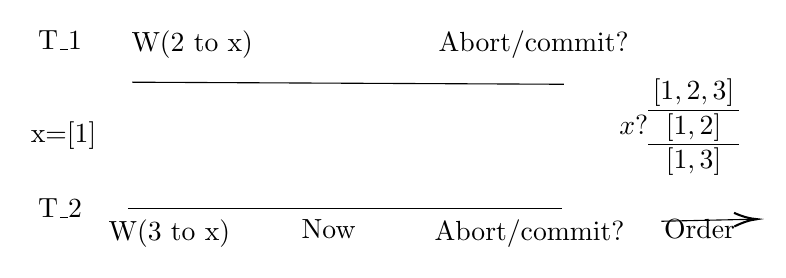
\begin{tikzpicture}[x=0.75pt,y=0.75pt,yscale=-1,xscale=1]
%uncomment if require: \path (0,300); %set diagram left start at 0, and has height of 300

%Straight Lines [id:da9500410641573396] 
\draw    (62.56,29) -- (270.56,30) ;
%Straight Lines [id:da7796185686481738] 
\draw    (60.56,90) -- (269.56,90) ;
%Straight Lines [id:da7329480179958066] 
\draw    (317.56,96) -- (361.56,95.04) ;
\draw [shift={(363.56,95)}, rotate = 178.75] [color={rgb, 255:red, 0; green, 0; blue, 0 }  ][line width=0.75]    (10.93,-3.29) .. controls (6.95,-1.4) and (3.31,-0.3) .. (0,0) .. controls (3.31,0.3) and (6.95,1.4) .. (10.93,3.29)   ;

% Text Node
\draw (16,3) node [anchor=north west][inner sep=0.75pt]   [align=left] {T\_1};
% Text Node
\draw (16,84) node [anchor=north west][inner sep=0.75pt]   [align=left] {T\_2};
% Text Node
\draw (61,3) node [anchor=north west][inner sep=0.75pt]   [align=left] {W(2 to x)};
% Text Node
\draw (50,94) node [anchor=north west][inner sep=0.75pt]   [align=left] {W(3 to x)};
% Text Node
\draw (209,3) node [anchor=north west][inner sep=0.75pt]   [align=left] {Abort/commit?};
% Text Node
\draw (207,94) node [anchor=north west][inner sep=0.75pt]   [align=left] {Abort/commit?};
% Text Node
\draw (317.56,94) node [anchor=north west][inner sep=0.75pt]   [align=left] {Order};
% Text Node
\draw (143,94) node [anchor=north west][inner sep=0.75pt]   [align=left] {Now};
% Text Node
\draw (12.5,47) node [anchor=north west][inner sep=0.75pt]   [align=left] {x=[1]};
% Text Node
\draw (296,25) node [anchor=north west][inner sep=0.75pt]   [align=left] {$x? \begin{array}{@{\,}c@{\,}}    [1,2,3]\\    \hline    [1,2]\\    \hline    [1,3]  \end{array} $};
\end{tikzpicture}
\vspace{2mm}

\subsection{P1 - Dirty Read}
The Dirty Read phenomena occurs when a transaction T2 Reads a object that has been modified by a concurrent transaction T1 prior to T1 committing or aborting. this results in t2 returning a object that might never have existed in the transaction history. The preventative interpretation for P1 uses the same locking of the history via long-term and short-term locks as P0, such that P1 requires T1 to acquire a long write-lock and T2 to acquire (at least) a short-term read-lock.

\subsubsection{Example of violation}
Suppose transaction T1 modifies a x by appending [2]. Transaction T2 then reads that x before T1 performs a COMMIT. If T1 then performs a ROLLBACK, T2 will have read x = [1,2] a object that was never committed and that may thus be considered to have never existed.\\
\vspace{5mm}
\tikzset{every picture/.style={line width=0.75pt}} %set default line width to 0.75pt        
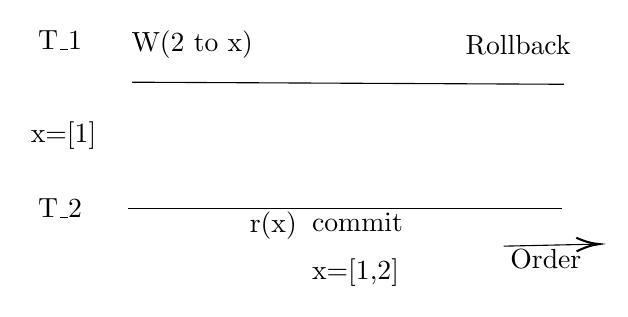
\begin{tikzpicture}[x=0.75pt,y=0.75pt,yscale=-1,xscale=1]
%uncomment if require: \path (0,300); %set diagram left start at 0, and has height of 300

%Straight Lines [id:da9500410641573396] 
\draw    (62.56,29) -- (270.56,30) ;
%Straight Lines [id:da7796185686481738] 
\draw    (60.56,90) -- (269.56,90) ;
%Straight Lines [id:da7329480179958066] 
\draw    (241.56,108) -- (285.56,107.04) ;
\draw [shift={(287.56,107)}, rotate = 178.75] [color={rgb, 255:red, 0; green, 0; blue, 0 }  ][line width=0.75]    (10.93,-3.29) .. controls (6.95,-1.4) and (3.31,-0.3) .. (0,0) .. controls (3.31,0.3) and (6.95,1.4) .. (10.93,3.29)   ;

% Text Node
\draw (16,3) node [anchor=north west][inner sep=0.75pt]   [align=left] {T\_1};
% Text Node
\draw (16,84) node [anchor=north west][inner sep=0.75pt]   [align=left] {T\_2};
% Text Node
\draw (61,3) node [anchor=north west][inner sep=0.75pt]   [align=left] {W(2 to x)};
% Text Node
\draw (118,90) node [anchor=north west][inner sep=0.75pt]   [align=left] {r(x)};
% Text Node
\draw (222,5) node [anchor=north west][inner sep=0.75pt]   [align=left] {Rollback};
% Text Node
\draw (148,91) node [anchor=north west][inner sep=0.75pt]   [align=left] {commit};
% Text Node
\draw (243.56,108) node [anchor=north west][inner sep=0.75pt]   [align=left] {Order};
% Text Node
\draw (12.5,47) node [anchor=north west][inner sep=0.75pt]   [align=left] {x=[1]};
% Text Node
\draw (148,113) node [anchor=north west][inner sep=0.75pt]   [align=left] {x=[1,2]};

\end{tikzpicture}
\newpage
\subsection{P2 - Non-repeatable/Fuzzy Read}
The occurrence of the P2 violation occurs when a given transaction T1 reads the same object multiple times and a given transaction T2 modifies this object in-between any of these reads causing T1 to see different versions of a object in the same transaction without modifying it itself. the preventative implementation for P2 requires the use of long read and write-locks; 

\subsubsection{Example of violation}
Suppose transaction T1 reads x as [1], transaction T2 then modifies x by appending 2 and commits. T1 then reads x as [1, 2].
\vspace{5mm}
 
\tikzset{every picture/.style={line width=0.75pt}} %set default line width to 0.75pt        
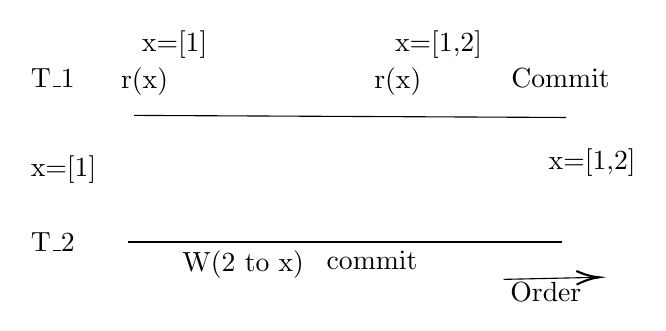
\begin{tikzpicture}[x=0.75pt,y=0.75pt,yscale=-1,xscale=1]
%uncomment if require: \path (0,300); %set diagram left start at 0, and has height of 300

%Straight Lines [id:da9500410641573396] 
\draw    (63.56,64) -- (271.56,65) ;
%Straight Lines [id:da7796185686481738] 
\draw    (60.56,125) -- (269.56,125) ;
%Straight Lines [id:da7329480179958066] 
\draw    (241.56,143) -- (285.56,142.04) ;
\draw [shift={(287.56,142)}, rotate = 178.75] [color={rgb, 255:red, 0; green, 0; blue, 0 }  ][line width=0.75]    (10.93,-3.29) .. controls (6.95,-1.4) and (3.31,-0.3) .. (0,0) .. controls (3.31,0.3) and (6.95,1.4) .. (10.93,3.29)   ;

% Text Node
\draw (12.5,40) node [anchor=north west][inner sep=0.75pt]   [align=left] {T\_1};
% Text Node
\draw (12.5,119) node [anchor=north west][inner sep=0.75pt]   [align=left] {T\_2};
% Text Node
\draw (85.56,128) node [anchor=north west][inner sep=0.75pt]   [align=left] {W(2 to x)};
% Text Node
\draw (56,40) node [anchor=north west][inner sep=0.75pt]   [align=left] {r(x)};
% Text Node
\draw (244,40) node [anchor=north west][inner sep=0.75pt]   [align=left] {Commit};
% Text Node
\draw (155,128) node [anchor=north west][inner sep=0.75pt]   [align=left] {commit};
% Text Node
\draw (243.56,143) node [anchor=north west][inner sep=0.75pt]   [align=left] {Order};
% Text Node
\draw (12.5,82) node [anchor=north west][inner sep=0.75pt]   [align=left] {x=[1]};
% Text Node
\draw (66,22) node [anchor=north west][inner sep=0.75pt]   [align=left] {x=[1]};
% Text Node
\draw (178,40) node [anchor=north west][inner sep=0.75pt]   [align=left] {r(x)};
% Text Node
\draw (188,22) node [anchor=north west][inner sep=0.75pt]   [align=left] {x=[1,2]};
% Text Node
\draw (262,79) node [anchor=north west][inner sep=0.75pt]   [align=left] {x=[1,2]};


\end{tikzpicture}

\subsection{P3 - Phantom Read}

The Phantom Read violation occurs when Transaction T1 preforms a conditional read operation. Following this initial read, a second transaction T2 either inserts or modifies objects such that they meet the conditional requirement of T1, T2 then commits this change. T1 then performs the same conditional read operation containing additional objects It is called Phantom Read because the new records seem to be of phantom origin. the preventative interpretation of P3 requires acquisition of long-term Phantom read-locks

\subsubsection{Example of violation}
Suppose Transaction T1 selects all values >= 2, Transaction T2 then writes 3 to key x and commits. T1 then selects all values >= 2. the object x now matches this predicate and is included in the read operation. \\
\vspace{5mm}
\tikzset{every picture/.style={line width=0.75pt}} %set default line width to 0.75pt        
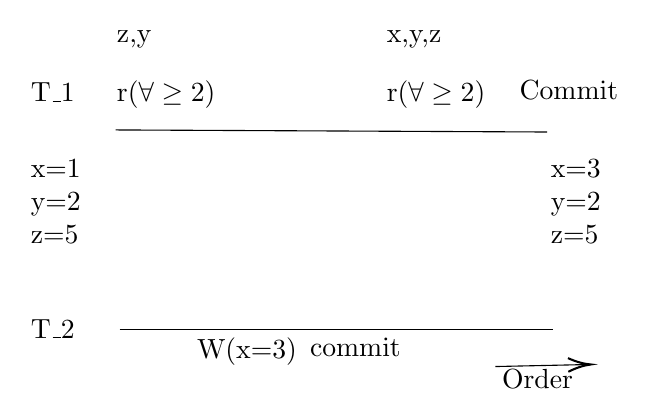
\begin{tikzpicture}[x=0.75pt,y=0.75pt,yscale=-1,xscale=1]
%uncomment if require: \path (0,300); %set diagram left start at 0, and has height of 300

%Straight Lines [id:da9500410641573396] 
\draw    (63.56,64) -- (271.56,65) ;
%Straight Lines [id:da7796185686481738] 
\draw    (65.56,160) -- (274.56,160) ;
%Straight Lines [id:da7329480179958066] 
\draw    (246.56,178) -- (290.56,177.04) ;
\draw [shift={(292.56,177)}, rotate = 178.75] [color={rgb, 255:red, 0; green, 0; blue, 0 }  ][line width=0.75]    (10.93,-3.29) .. controls (6.95,-1.4) and (3.31,-0.3) .. (0,0) .. controls (3.31,0.3) and (6.95,1.4) .. (10.93,3.29)   ;

% Text Node
\draw (21.5,40) node [anchor=north west][inner sep=0.75pt]   [align=left] {T\_1};
% Text Node
\draw (21.5,154) node [anchor=north west][inner sep=0.75pt]   [align=left] {T\_2};
% Text Node
\draw (101.56,163) node [anchor=north west][inner sep=0.75pt]   [align=left] {W(x=3)};
% Text Node
\draw (63,39) node [anchor=north west][inner sep=0.75pt]   [align=left] {r($\forall \geq 2$)};
% Text Node
\draw (257,39) node [anchor=north west][inner sep=0.75pt]   [align=left] {Commit};
% Text Node
\draw (156,163) node [anchor=north west][inner sep=0.75pt]   [align=left] {commit};
% Text Node
\draw (248.56,178) node [anchor=north west][inner sep=0.75pt]   [align=left] {Order};
% Text Node
\draw (21.5,77) node [anchor=north west][inner sep=0.75pt]   [align=left] {x=1\\y=2\\z=5};
% Text Node
\draw (193,15) node [anchor=north west][inner sep=0.75pt]   [align=left] {x,y,z};
% Text Node
\draw (63,15) node [anchor=north west][inner sep=0.75pt]   [align=left] {z,y};
% Text Node
\draw (193,39) node [anchor=north west][inner sep=0.75pt]   [align=left] {r($\forall \geq 2$)};
% Text Node
\draw (272,77) node [anchor=north west][inner sep=0.75pt]   [align=left] {x=3\\y=2\\z=5};

\end{tikzpicture}
    
\newpage
\subsection{Currently Described Anomalies} \todo[author=Mark]{ Unsure what to name this.}

Following the ANSI standard and Adya et al\cite{Adya99weakconsistency} a significant amount of discoveries have been made that describes anomalies not accounted for in most definitions of consistency models. A recent paper by Haixiang Li et al\cite{li2021coo} describes a total of 18 anomalies either described in standards or paper in the past 30 years, The paper mentions that all these definitions are defined Case by case and not in a rigours mathematically manner. The paper includes the following sentence: 
\begin{quote}
    "Definition of data anomalies. Although there are so many data anomalies, but it seems that data anomalies are not explicitly defined. There is no universally accepted definition of data anomalies in academia and industry, and the understanding of data anomalies is only in the way of case-by-case" \cite{li2021coo}
\end{quote}

The 18 transactional anomalies are listed below. These definitions will not be explored deeper unless relevant for the thesis.

\begin{table}[h]
    \begin{tabular}{l|l|l}
        No & Anomaly, reference, year                        & Formal definition  \\ \hline
        1  & Dirty Write {[}1{]} 1992                        & $W_1 [x_1 ]...W_2 [x_2 ]...((C_1 or A_1) and (C_2 or A_2) in any order) $  \\
        2  & Lost Update {[}6{]} 1995                        & $  R_1 [x_0 ]...W_2 [x_1 ]...C_2...W_1 [x_2 ] $ \\
        3  & Dirty Read {[}1{]} 1992                         & $ W_1 [x ]...R_2 [x ]...(A_1 and C_2 in either order) $ \\
        4  & Aborted Reads {[}45{]} 2015, {[}2{]} 2000       & $ W_1 [x : i]...R_2 [x : i]...(A_1 and C_2 in any order) $  \\
        5  & Fuzzy/Non-repeatable Read {[}1{]} 1992          & $ R_1 [x ]...W_2 [x ]...C_2...R_1 [x ]...C_1 $  \\
        6  & Phantom {[}1{]} 1992                            & $ R_1 [P ]...W_2[y in P]...C_2...R_1 [P ]...C_1 $  \\
        7  & Intermediate Reads {[}45{]} 2015, {[}2{]} 2000  & $ W_1 [x : i]...R_2 [x : i]...W_1 [x : j]...C_2  $  \\
        8  & Read Skew {[}6{]} 1995                          & $ R_1 [x_0 ]...W_2 [x_1 ]...W_2 [y_1 ]...C_2...R_1 [y_1] $ \\
        9  & Unnamed Anomaly {[}38{]} 2000                   & \begin{tabular}[c]{@{}l@{}}$ R_1 [y]...R_2 [x ]...W_2 [x ]...R_2 [y]...W_2 [y]...C_2...R_3 [x ]...W_3 [x ]$\\$...R_3 [z]...W_3 [z]...C_3...R_1 [z]...C_1 $\end{tabular}      \\
        10 & Fractured Reads {[}16{]} 2017, {[}5{]} 2014     & $ R_1 [x_0]...W_2 [x_1 ]...W_2 [y_1 ]...C_2...R_1 [y_1 ] $ \\
        11 & Serial-Concurrent-phenomenon {[}12{]} 2014      & $ R_1 [x_0 ]...W_2 [x_1 ]...W_2 [y_1 ]...C_2...R_1 [y_1 ] $  \\
        12 & Cross-phenomenon {[}12{]} 2014                  & $ R_1 [x_0 ]...R_2 [y_0 ]...W_3 [x_1 ]...C_3...W_4 [y_1 ]...C_4...R_2 [x_1 ]...R_1 [y_1 ] $ \\
        13 & Long Fork Anomaly {[}16{]} 2017                 & $ R_1 [x_0 ]...R_2 [y_0 ]...W_3 [x_1 ]...C_3...W_4 [y_1 ]...C_4...R_2 [x_1 ]...R_1 [y_1 ] $ \\
        14 & Causality Violation Anomaly {[}16{]} 2017       & $ R_1 [x_0 ]...W_2 [x_1 ]...C_2...R_3 [x_1 ]...W_3 [y_1 ]...C_3...R_1 [y_1 ] $  \\
        15 & Read-only Transaction Anomaly {[}26, 43{]} 2004 & \begin{tabular}[c]{@{}l@{}}$ R_1 [x_0, 0]...R_1 [y_0, 0]...R_2 [y_0, 0]...W_2 [y_1, 20]...C_2$\\$...R_3 [x_0,0]...R_3 [y_1, 20]...C_3...W_1 [x_2, -11]...C_1 $\end{tabular} \\
        16 & Write Skew {[}6{]} 1995                         & $ R_1 [x_0 ]...R_2 [y_0 ]...W_1 [y_1 ]...W_2 [x_1 ] $   \\
        17 & Predicate-based Write Skew {[}27{]} 2005        & $ R_1 [P ]...R_2 [P ]...W_1 [y_1 in P]...W_2[x_1 in P] $  \\
        18 & Read Partial-Committed {[}44{]} 2019            & $ R_1[x] W_2[x] W_2[y] C_2 R_1[Y] C_1 $ 
    \end{tabular}
\end{table}

\vspace{5mm}

Outside of the above paper other anomalies and issues exist within databases, a deeper investigation into these won't take place but a short explanation will be given here for issues that occur often to create awareness about the issue,
\begin{itemize}
    \item Split Brain, A Split Brain occurs when a distributed Database is partitioned in 2 of more fragments that are unable to reach each other but both remain active with a new leader and continue to process transaction, This leads to each fragment believing in separate histories, and is a regular occurrence in distributed databases.\cite{aphyrelasticsearch, jepsenscylla, jepsenhazelcast}, Some systems can recover from this but often loose data during the healing process.
    \item Poor handling of quorum
\end{itemize}

\newpage
\section{Consistency models}


\begin{wrapfigure}{r}{0.5\linewidth}
    \centering
    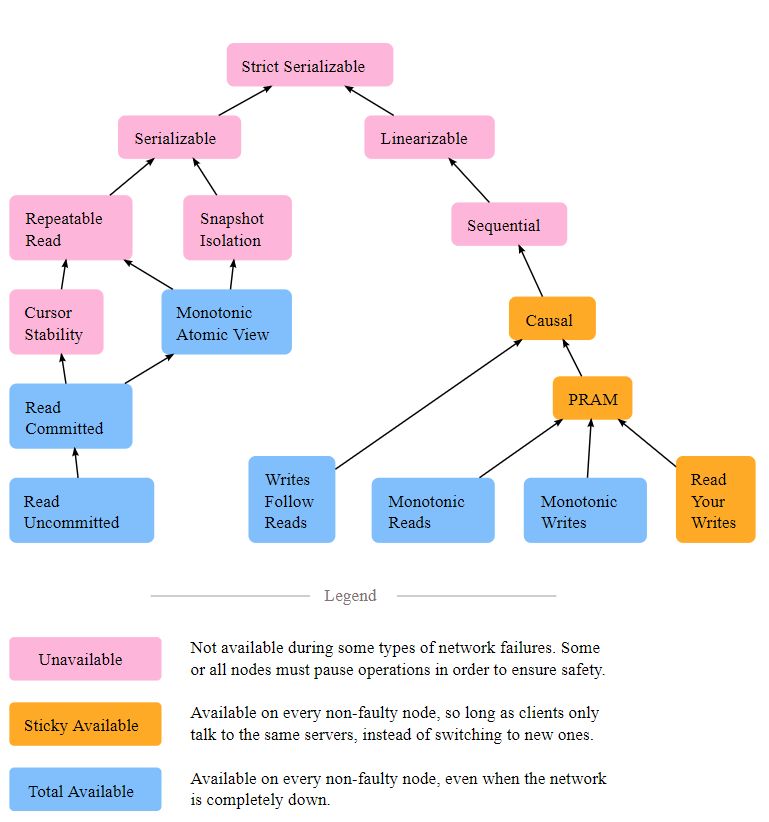
\includegraphics[scale=0.4]{images/consistency models.PNG}
    \caption{Picture from jepsen.io/consistency}
    \label{fig:jepsenioconsistency}
\end{wrapfigure}

For explaining the concepts within consistency, I will use a paper by Ballis et al. on "Highly available transactions"\cite{HighlyAvailableTransactionsVirtuesandLimitations} that contains a good model for presenting the different consistency models and their relation to other consistency models. A focus will be on Transactional models so not all of the BASE models are covered.\\

\subsection{Strict Serializability}

For a system to have Strict Serializability, it is required that the entire system operationally appears to occur in order, with regards to both the order and the real-time of the operations. Within the CAP theorem, this would be considered a CA system.\\
\vspace{5mm}
Formally Strict Serializability is defined as a Serviceable system that is compatible with a Time-dependent order.
"A history is serializable if it is equivalent to one in which transactions appear to execute sequentially, i.e., without interleaving. A (partial) precedence order can be defined on non-overlapping pairs of transactions in an obvious way. A history is strictly serializable if the transactions' order in the sequential history is compatible with their precedence order." \cite{Herlihy1990Linearizability}\\
\vspace{5mm}
Here it should be clarified what is menat by the obvious way" is for a transactions A and B, that A proceeds B if A completes prior to transaction B's begin or in other words a Serializable system with the time constraint from Linearizability.

SS cannot be totally or sticky available in the event of a network partition. In this case, some or all nodes will be stuck; this is due to the nature of the Strict Serializable consistency model, where transactions operate on the system as a whole, as in the case of a partition in the distributed system, this is impossible. There can be cases where replicate nodes are partitioned from the primary nodes, and the primary nodes can continue with some degradation but where the replicas either shut down or serve stale data. In the case of primary nodes partitioning, the system would be unable to resume due to not being able to commit a given transaction to the entire system.


\begin{table}[h]
    \begin{tabular}{l|l|l|l}
        T1   & T2   & T3   & T4   \\
        w(1) &      &      &      \\
        r(2) &      &      &      \\
        c    &      &      &      \\
        & r(1) &      &      \\
        & r(2) &      &      \\
        & c    &      &      \\
        &      & r(3) &      \\
        &      & w(4) &      \\
        &      & c    &      \\
        &      &      & r(1) \\
        &      &      & c
    \end{tabular}
    \caption{Transactions are ordered chronological in time, and executed as such.}
\end{table}

\subsection{Serializable transaction models}

\subsubsection{Serializable}

Serializability is a relaxation of the Strict Serializability consistency model that foregoes that real-time constraint. It defines systems where transactions occur in some total order. It is formally defined in the ANSI SQL 1999 spec as follows.

\begin{quote}
"The execution of concurrent SQL-transactions at isolation level SERIALIZABLE is guaranteed to be serializable. A serializable execution is defined to be an execution of the operations of concurrently executing SQL-transactions that produces the same effect as some serial execution of those same SQL-transactions. A serial execution is one in which each SQL-transaction executes to completion before the next SQL-transaction begins."\cite{ansisql1999}\\
\end{quote}
\vspace{5mm}

The above implies that Serializability of the transactions does not only apply to the objects in use but the system as a whole. This means that in the case of a network partition some or all notes will be stuck until the network is healed. Further, as no real-time constraint is enforced,  we can observe stale reads. This occurs when process A completes a write, then process B begins a read, and the read is not guaranteed to observe the write from process A.
\\ \vspace{5mm}

There is a further limitation of Serializable due to having no real-time constraint; SR allows pathological orderings. This allows a serializable database to discard, write, and increment operations that are never observed by executing them at the very end of the history. Furthermore, read operations can always return an empty state by placing the transaction at the beginning of the history. It should however be noted that most implementation does not take advantage of this.
\\ \vspace{5mm}
SR follows closely to S-SR regarding partition tolerance and availability doing partition and is therefore considered a CA database.
\\ \vspace{5mm}
\begin{table}[h]
    \begin{tabular}{l|l|l|l}
        T1   & T2   & T3   & T4   \\
        w(z) &      &      &      \\
        & r(z) &      &      \\
        &      &      & r(z) \\
        & w(y) &      &      \\
        &      &      & c    \\
        &      & r(y) &      \\
        & c    &      &      \\
        &      & w(h) &      \\
        r(x) &      &      &      \\
        c    &      &      &      \\
        &      & c    &
    \end{tabular}
    \caption{Transactions are ordered chronological in time and executed in a way that makes it possible for the operations to occur atomically such that they appear to have been executed in order transaction-wise. }
\end{table}
\newpage

\subsubsection{Repeatable Read}

Repeatable Read (RR) closely resembles the Serializable consistency model, however in RR we allow phantoms. This implies that if T1 reads a predicate like "select all from alarms with the newest timestamp," another transaction T2 is able to create or modify values within the predicate before T1 commits. So if the transaction T1 performs the read again, this predicate might not be stable.
\\ \vspace{5mm}
RR contains the above relaxation; however, this relaxation implies more than meets the eye. For example, repeatable read doesn't guarantee repeatable reads in the sense that we might consider. This is due to RR not requiring any real-time constraint; this allows for a situation where process A performs a write, and after process A completes process B performs a read. However, this read is not guaranteed to obverse the write from process A. Furthermore, as no per-process ordering of transactions is required, process A can write something and then fail to observe that write in a subsequent transaction.
\\ \vspace{5mm}
It should also be noted that RR allows for the same pathological ordering of operations as a Serializable database.

\begin{table}[h]
    \begin{tabular}{l|l|l|l}
        T1            & T2            & T3   & T4   \\
        &               &      & r(y) \\
        &               &      & c    \\
        w(p$_1$ to y) &               &      &      \\
        r(p in y)     &               &      &      \\
        &               &      &      \\
        & w(p$_2$ to y) &      &      \\
        & c             &      &      \\
        r(p in y)     &               &      &      \\
        w(z)          &               &      &      \\
        c             &               &      &      \\
        &               & r(z) &      \\
        &               & w(x) &      \\
        &               & c    &
    \end{tabular}
    \caption{T1 shows an example of a valid transaction with a phantom, and T4 could be placed at the beginning of the history, returning the "empty" result. Both are valid transactions within RR.}
\end{table}

\subsection{Cursor Stability}
Cursor Stability closely resembles repeatable read where RR locks the objects until committed. Cursor Stability locks the objects until the cursor moves on or until committed. This allows for different behavior depending on implementation but is formally defined by which phenomena it allows and which it prohibits. \cite{Adya99weakconsistency}\\
\begin{itemize}
    \item G-cursor(x): the directed serialization graph, restricted to a single object x, contains an anti-dependency cycle and at least one write-dependency edge.
    \item g1:
    \begin{enumerate}
        \item G1a (Aborted Reads): A transaction observes an object (perhaps via a predicate) modified by an aborted transaction. Intuitively, transactions have to commit for us to read them.
        \item G1b (Intermediate Reads): A transaction observes an object (perhaps via a predicate) modified by a transaction that was not that transaction's final modification of that object. Intuitively, transactions have to finish before we can read them,
        \item G1c (Circular Information Flow): the Directed Serialization Graph of transactions contains a directed cycle consisting entirely of dependency edges. Intuitively, if transaction T1 is affected by T2, T2 can't be affected by T1.
    \end{enumerate}
\end{itemize}
Furthermore, since cursor stability is strictly stronger than read committed, it also prohibits the ANSI phenomena:
\begin{itemize}
    \item P0 (Dirty Write): w1(x) … w2(x)
    \item P1 (Dirty Read): w1(x) … r2(x)
\end{itemize}

but allows:
\begin{itemize}
    \item P2 (Fuzzy Read): r1(x) … w2(x)
    \item P3 (Phantom): r1(P) … w2(y in P)
\end{itemize}


\todo[author=Mark]{Make diagram Cursor Stability}

\subsection{Snapshot Isolation}

Snapshot Isolation behaves differently to any of the systems. It can be considered more as a \textbf{try: commit() catch: abort()} . We perform our transaction in an independent branch and commit/merge to the database on commit; if there are any conflicts with an already committed transaction, the transaction is simply aborted.
\\ \vspace{5mm}
Snapshot Isolation, like Readable Read, operates on an object level and allows for the same behavior. Items are stable once read; however, the predicate again isn't. We can fail to observe a previously committed transaction and place operations in arbitrary places in the transaction due to no Linearizability constraint. It also allows sub-operations to interleave. This can result in write skews, which allow transactions to read overlapping states, modify disjoint sets of objects, then commit; and a read-only transaction anomaly involving partially disjointing write sets.
\\ \vspace{5mm}

It should also be noted that there exist multiple versions of Snapshot Isolation, one being prefix-consistent snapshot isolation that enforces process-level transaction ordering, which prevents a given process from failing to observe a previous transaction; and another being parallel snapshot isolation that allows for total availability but this allows for long fork anomalies, as each node has its own transaction ordering.
\\ \vspace{5mm}
Formally Snapshot Isolation is defined by Berenson et al.\cite{Berensonetal}. as:

\begin{displayquote}
… each transaction reads data from a snapshot of the (committed) data as of the time the transaction started, called its Start-Timestamp. This time may be any time before the transaction's first Read. A transaction running in Snapshot Isolation is never blocked attempting a read as long as the snapshot data from its Start-Timestamp can be maintained. The transaction's writes (updates, inserts, and deletes) will also be reflected in this snapshot, to be read again if the transaction accesses (i.e., reads or updates) the data a second time. Updates by other transactions active after the transaction Start-Timestamp are invisible to the transaction.
\\
When the transaction T1 is ready to commit, it gets a Commit-Timestamp, larger than any existing Start-Timestamp or Commit-Timestamp. The transaction successfully commits only if no other transaction T2 with a Commit-Timestamp in T1's execution interval [StartTimestamp, Commit-Timestamp] wrote data that T1 also wrote. Otherwise, T1 will abort. This feature, called First-committer-wins prevents lost updates (phenomenon P4). When T1 commits, its changes become visible to all transactions whose Start-Timestamps are larger than T1's Commit-Timestamp.
\end{displayquote}


There also exist multiple other definitions from Cerone et al \cite{CeroneBernardiGotsman} and Crooks et al\cite{CrooksPuAlvisiClement}


\begin{table}[h]
    \begin{tabular}{l|l|l|l}
        T1   & T2   & T3   & T4   \\
        &      &      & r(y) \\
        &      &      & c    \\
        w(y) &      &      &      \\
        r(y) &      &      &      \\
        &      &      &      \\
        & w(y) &      &      \\
        &      &      &      \\
        r(y) &      &      &      \\
        w(z) &      &      &      \\
        c    &      &      &      \\
        & a    & r(z) &      \\
        &      & w(x) &      \\
        &      & c    &
    \end{tabular}
    \caption{T1 and T2 contains a conflict that courses T2 to abort as T1 commits prior to T2}
\end{table}



\subsubsection{Monotonic Atomic View}
The Monotonic Atomic view(MAV) model is a relaxation of snapshot isolation. It requires that effects by transactions are fully visible once read by other transactions, such that T1 may preform w(1), w(2), w(2), c. These 3 sub operations effects should all either be fully visible or not at all, so partial transactions aren't allowed. Formally this is defined by Bailis et al \cite{HighlyAvailableTransactionsVirtuesandLimitations}
\textit{Under MAV, once some of the effects of a transaction Ti are observed by another transaction Tj, thereafter, all effects of Ti are observed by Tj. That is, if a transaction Tj reads a version of an object that transaction Ti wrote, then a later read by Tj cannot return a value whose later version is installed by Ti.}

and by Adya et al\cite{Adya99weakconsistency} as prohibiting:
\begin{itemize}
    \item G1b (Intermediate Reads): A transaction observes an object (perhaps via a predicate) modified by a transaction that was not that transaction's final modification of that object. Intuitively, transactions have to finish before we can read them,
\end{itemize}

Further since MAV is strictly stronger than Read Committed, it also disallows the ANSI phenomena Dirty Write(P0), Dirty Read (P1) but allows Fuzzy Read (P2) and Phantom (P3)

\subsection{Read Committed}
The Read Committed transaction model is the first non-atomic transaction model where partial visibility of committed transactions is permitted. This however might lead to foreign key constraint issues, among other problems where required data joins are performed due to not yet visible values.
\\ \vspace{5mm}

Formally it is defined in ANSISQL1999\cite{ansisql1999} by disallowing P1
\textit{P1 ("Dirty read" ): SQL-transaction T1 modifies a row. SQL-transaction T2 then reads that row before T1 performs a COMMIT. If T1 then performs a ROLLBACK, T2 will have read a row that was never committed and that may thus be considered to have never existed.} However, in the Microsoft paper, Berenson et al \cite{Berensonetal} it is observed that the ANSI specification allows multiple interpretations, one of which allows non-serializable histories. Here Adya et al.\cite{Adya99weakconsistency} is commonly used as it provides a concrete specification based on the unconcise ANSI specification.
\\ \vspace{5mm}

\todo[author=Mark]{TODO Make Diagram Read committed}

\subsection{Read Uncommitted}
Read Uncommitted as defined by ANSI allows all behavior. However, this has been challenged by Berenson et al\cite{Berensonetal} where they argue that Read Uncommitted should disallow dirty writes. This is also the non-ANSI defacto definition as per Adya et al \cite{Adya99weakconsistency} which again provides a better definition based, on what can be interpreted from the loose definition in ANSISQL99\cite{ansisql1999}. It should be noted that due to the loose specification in ANSI, multiple mainstream interpretations exist.\\

by the Aday's specification Read Uncommitted disallows
\begin{itemize}
    \item Dirty Write(P0)
\end{itemize}
But allows
\begin{itemize}
    \item Dirty read(P1)
    \item Fuzzy Read (P2)
    \item Phantom (P3)
\end{itemize}

\subsection{Non-transaction models (BASE)}
The category of BASE transaction models aren't considering the order of transactions but rather the ordering of operations in real time. Only Linearizable and Sequential Consistency is introduced here. other BASE models exist, The core ones are Casual Consistency, Writes Follows Reads, Monotonic Reads, Monotonic Writes and Read your writes.

\subsubsection{Linearizable}
Linearizablilty is the strongest single object consistency model, that requires operations to occur in a order consistent with real time, and the operations themselves should occur atomically. It should also be noted that linearzability is not tolerant to network partitions and should be considered a CA model according to the CAP theorem.

it is formalized  in \cite{Linearizability} and later specified  in \cite{ConsistencyinNonTransactionalDistributedStorageSystems} where it's defined by 3 requirements

\begin{itemize}
    \item Single Order (there exists some total order of operations)
    \item RealTime (consistent with the real time bound)
    \item RVal (obeying the single-threaded laws of the associated object's datatype)
\end{itemize}

\subsubsection{Sequential Consistency}
Sequential Consistency (SC) is a relaxation of Linearizability. Unlike Linearizability, SC is a concurrent model. Here the requirement is that all operations follow a total order and this order is consistent across all processes. However, since a Total order is required, the model is unable to tolerate partitions and some or all nodes will be unable to make progress. 
\\ \vspace{5mm}
One of the phenomena SC allows is Stale Reads. All processes have to follow the same total order but as there isn't a strong constraint concerning how far a process may be behind or ahead and it may return an arbitrarily stale state. However, once a given node A observes some operations from a separate node B, A may never observe a state prior to B.

Formally SC was defined by Leslie Lamport\cite{Lamport1979how}, however Viotti and Vukolić\cite{ConsistencyinNonTransactionalDistributedStorageSystems} formalized it into three requirements:
\begin{itemize}
    \item SingleOrder (there exists some total order of operations)
    \item PRAM (the session order (the order of operations on each process) is a subset of the visibility order (what operations are visible to a given operation).)
    \item RVal (the order must be consistent with the semantics of the datatype)
\end{itemize}

\todo[author=Mark]{Two of the consistency models were already mentioned in the previous section namely Atomic Consistency and Sequential Consistency. There exist two more models within common use, which are Causal Consistency and Eventual Consistency. They differ in the way the consistency is handled by all end up in the same state eventually.}



\section{Directed Serialization graphs}

Directed Serialization graphs(DSG) are to reason about a history of Transactions and operations within a transaction, such that each node represents a node and edges represent different types of direct conflicts. \\ using these conflicts we can reason about what order transactions were executed in and if any transactional phenomena of anomalies occurred. These are defined in terms of DSG cycles and conflict relations. 
\subsection{Transaction conflicts relations}
\subsubsection{Read-dependency}

The Read-dependency is when a Transaction $T_j$ directly depends on a write from a transaction $T_i$ where $T_i$ writes some object $x_i$ and $T_j$ reads $x_i$, this relation is also called Write-Read (wr) as one transaction writes a object and a second transaction depends on this prior write.
        
\tikzset{every picture/.style={line width=0.75pt}} %set default line width to 0.75pt        

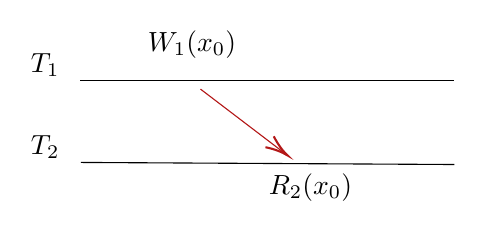
\begin{tikzpicture}[x=0.75pt,y=0.75pt,yscale=-1,xscale=1]
%uncomment if require: \path (0,300); %set diagram left start at 0, and has height of 300

%Straight Lines [id:da9351620672631715] 
\draw    (70.33,79.67) -- (250.33,79.67) ;
%Straight Lines [id:da20316716985592453] 
\draw    (70.67,119.33) -- (250.67,120.33) ;
%Straight Lines [id:da3663864520178606] 
\draw [color={rgb, 255:red, 179; green, 23; blue, 23 }  ,draw opacity=1 ]   (128.33,84) -- (168.74,114.79) ;
\draw [shift={(170.33,116)}, rotate = 217.3] [color={rgb, 255:red, 179; green, 23; blue, 23 }  ,draw opacity=1 ][line width=0.75]    (10.93,-3.29) .. controls (6.95,-1.4) and (3.31,-0.3) .. (0,0) .. controls (3.31,0.3) and (6.95,1.4) .. (10.93,3.29)   ;

% Text Node
\draw (45.33,65.67) node [anchor=north west][inner sep=0.75pt]   [align=left] {$T_1$};
% Text Node
\draw (45.33,105) node [anchor=north west][inner sep=0.75pt]   [align=left] {$T_2$};
% Text Node
\draw (101.67,54.67) node [anchor=north west][inner sep=0.75pt]   [align=left] {$W_1(x_0)$};
% Text Node
\draw (160,123.67) node [anchor=north west][inner sep=0.75pt]   [align=left] {$R_2(x_0)$};


\end{tikzpicture}

We have a history H. as follows.
\begin{equation}
    History\ H: [T_1(W(x_0)), T_2(R(x_0))]
\end{equation}

This history contains two transactions $T_i$ followed by $T_j$. $T_i$ writes version $x_0$, which is later read by $T_j$, thus item-read-depends on $T_i$. this wr is also denoted by the red arrow in the above illustration.
    
A SQL example of this relation would be the below script
        
\begin{lstlisting}
update accounts set balance = 42 where id = 1;
select * from accounts where id = 1;
\end{lstlisting}
        
        

\subsubsection{predicate-based read dependency (wr)}
A Predicate read dependency occurs when a transactions $T_j$ preforms a operation containing multiple reads while a concurrent $T_i$ is preforming writes within the predicate of $T_j$. This occurs if $T_i$ write $x_i$, $x_h$ precedes $x_i$ in the history, and $x_h$ matches Predicate where $x_i$ does not or opposite were $x_h$ does not match the predicate whereas $x_i$ does.\\

This case of WR dependency gives the symptom of objects appearing or disappearing within a transaction. 


\tikzset{every picture/.style={line width=0.75pt}} %set default line width to 0.75pt        

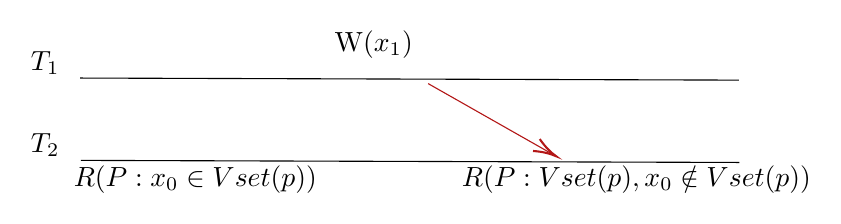
\begin{tikzpicture}[x=0.75pt,y=0.75pt,yscale=-1,xscale=1]
%uncomment if require: \path (0,300); %set diagram left start at 0, and has height of 300

%Straight Lines [id:da9351620672631715] 
\draw    (41.33,82) -- (358.67,83) ;
%Straight Lines [id:da20316716985592453] 
\draw    (41.67,121.67) -- (359,122.67) ;
%Straight Lines [id:da3663864520178606] 
\draw [color={rgb, 255:red, 179; green, 23; blue, 23 }  ,draw opacity=1 ]   (209,84.67) -- (268.93,118.68) ;
\draw [shift={(270.67,119.67)}, rotate = 209.58] [color={rgb, 255:red, 179; green, 23; blue, 23 }  ,draw opacity=1 ][line width=0.75]    (10.93,-3.29) .. controls (6.95,-1.4) and (3.31,-0.3) .. (0,0) .. controls (3.31,0.3) and (6.95,1.4) .. (10.93,3.29)   ;

% Text Node
\draw (16.33,68) node [anchor=north west][inner sep=0.75pt]   [align=left] {$T_1$};
% Text Node
\draw (16.33,107.33) node [anchor=north west][inner sep=0.75pt]   [align=left] {$T_2$};
% Text Node
\draw (162.67,58) node [anchor=north west][inner sep=0.75pt]   [align=left] {W($x_1$)};
% Text Node
\draw (224,123) node [anchor=north west][inner sep=0.75pt]   [align=left] {$R(P:Vset(p),x_0\notin Vset(p)$)};
% Text Node
\draw (37,123) node [anchor=north west][inner sep=0.75pt]   [align=left] {$R( P:x_0 \in Vset(p))$};


\end{tikzpicture}

Transaction $T_2$ sees $x_0$ in it's first predicate read, however in the second read nothing is observed as $x_0$ was overwritten by $x_1$ via $T_1$. \\

We have a history H. as follows.
\begin{equation}
    History\ H: [T_1(W(x_1)), T_2(R(x_0),R(\emptyset))]
\end{equation}

A SQL example of this relation would be the below script

\begin{lstlisting}
select * from accounts where balance > 0;
update accounts set balance = -42 where id = 1;
select * from accounts where balance > 0;
\end{lstlisting}
        
        
\subsubsection{Write-dependency (ww)}
A write dependency occurs when transaction $T_j$ directly depends on $T_i$ if $T_i$ writes $x_i$, and $T_j$ writes the version of x following $T_i$ in the history. the relation is named ww as two writes to the same object with only one persisting.


\tikzset{every picture/.style={line width=0.75pt}} %set default line width to 0.75pt        

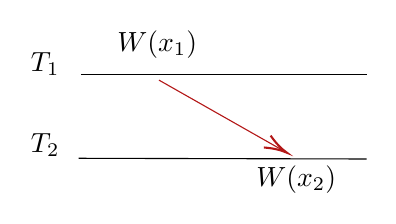
\begin{tikzpicture}[x=0.75pt,y=0.75pt,yscale=-1,xscale=1]
%uncomment if require: \path (0,300); %set diagram left start at 0, and has height of 300

%Straight Lines [id:da9351620672631715] 
\draw    (41.67,80) -- (179.67,80) ;
%Straight Lines [id:da20316716985592453] 
\draw    (40.67,120.33) -- (179.33,120.67) ;
%Straight Lines [id:da3663864520178606] 
\draw [color={rgb, 255:red, 179; green, 23; blue, 23 }  ,draw opacity=1 ]   (79.33,82.67) -- (139.26,116.68) ;
\draw [shift={(141,117.67)}, rotate = 209.58] [color={rgb, 255:red, 179; green, 23; blue, 23 }  ,draw opacity=1 ][line width=0.75]    (10.93,-3.29) .. controls (6.95,-1.4) and (3.31,-0.3) .. (0,0) .. controls (3.31,0.3) and (6.95,1.4) .. (10.93,3.29)   ;

% Text Node
\draw (16.33,68) node [anchor=north west][inner sep=0.75pt]   [align=left] {$T_1$};
% Text Node
\draw (16.33,107.33) node [anchor=north west][inner sep=0.75pt]   [align=left] {$T_2$};
% Text Node
\draw (58,57.67) node [anchor=north west][inner sep=0.75pt]   [align=left] {$W(x_1)$};
% Text Node
\draw (125,122.67) node [anchor=north west][inner sep=0.75pt]   [align=left] {$W(x_2)$};
\end{tikzpicture}

Transaction $T_2$ overwrites the object $x_1$ written by $T_1$ implying a Write-depends on $T_1$, The dependency is denoted by the red arrow in the graph. \\

\begin{equation}
    History\ H: [T_1(W(x_1)), T_2(W(x_2))]
\end{equation}

A SQL example of this relation would be the below script

\begin{lstlisting}
update accounts set balance = 42 where id = 42;
update accounts set balance = -42 where id = 42;
\end{lstlisting}

\subsubsection{Anti-dependency (rw)}
An read-write-dependency, or formally known as a anti-dependency occurs when a transaction overwrites a version observed by some other transaction. i.e. transaction T1 reads an object x, x is then modified by transaction T2.


\tikzset{every picture/.style={line width=0.75pt}} %set default line width to 0.75pt        

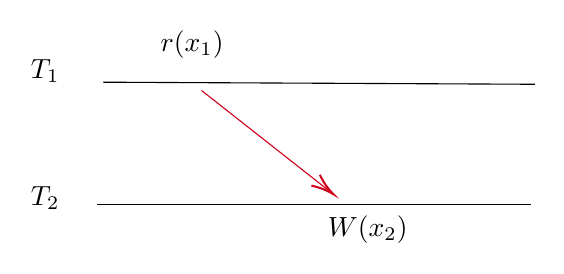
\begin{tikzpicture}[x=0.75pt,y=0.75pt,yscale=-1,xscale=1]
%uncomment if require: \path (0,300); %set diagram left start at 0, and has height of 300

%Straight Lines [id:da9500410641573396] 
\draw    (50.56,42) -- (258.56,43) ;
%Straight Lines [id:da7796185686481738] 
\draw    (47.56,101) -- (256.56,101) ;
%Straight Lines [id:da9563274467788809] 
\draw [color={rgb, 255:red, 208; green, 2; blue, 27 }  ,draw opacity=1 ]   (98,46) -- (159.99,94.76) ;
\draw [shift={(161.56,96)}, rotate = 218.19] [color={rgb, 255:red, 208; green, 2; blue, 27 }  ,draw opacity=1 ][line width=0.75]    (10.93,-3.29) .. controls (6.95,-1.4) and (3.31,-0.3) .. (0,0) .. controls (3.31,0.3) and (6.95,1.4) .. (10.93,3.29)   ;

% Text Node
\draw (14.5,30) node [anchor=north west][inner sep=0.75pt]   [align=left] {$T_1$};
% Text Node
\draw (14.5,91) node [anchor=north west][inner sep=0.75pt]   [align=left] {$T_2$};
% Text Node
\draw (157.56,105) node [anchor=north west][inner sep=0.75pt]   [align=left] {$W(x_2)$};
% Text Node
\draw (77,16) node [anchor=north west][inner sep=0.75pt]   [align=left] {$r(x_1)$};


\end{tikzpicture}

Transaction $T_1$ reads $X_1$, this object is then modified by $T_2$ and therefor anti-depends on $T_1$, i,e $T_2$ occurred after $T_1$ in the history.
\begin{equation}
    History\ H: [T_1(r(x_0)), T_2(W(x_1))]
\end{equation}


A SQL example of this relation would be the below script:
\begin{lstlisting}
  select * from accounts where id = 42;
  update accounts set balance = 2022 where id = 42;
\end{lstlisting}

\subsection{phenomena defined via cycles and conflicts}

\subsection{G0: dirty writes}
A history exhibits phenomenon G0 if the DSG contains a directed cycle consisting entirely of write-dependency edges.

\tikzset{every picture/.style={line width=0.75pt}} %set default line width to 0.75pt        




\tikzset{every picture/.style={line width=0.75pt}} %set default line width to 0.75pt        

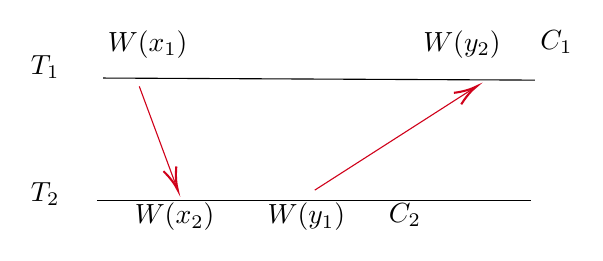
\begin{tikzpicture}[x=0.75pt,y=0.75pt,yscale=-1,xscale=1]
%uncomment if require: \path (0,300); %set diagram left start at 0, and has height of 300

%Straight Lines [id:da9500410641573396] 
\draw    (50.56,42) -- (258.56,43) ;
%Straight Lines [id:da7796185686481738] 
\draw    (47.56,101) -- (256.56,101) ;
%Straight Lines [id:da9563274467788809] 
\draw [color={rgb, 255:red, 208; green, 2; blue, 27 }  ,draw opacity=1 ]   (68,46) -- (85.86,94.13) ;
\draw [shift={(86.56,96)}, rotate = 249.64] [color={rgb, 255:red, 208; green, 2; blue, 27 }  ,draw opacity=1 ][line width=0.75]    (10.93,-3.29) .. controls (6.95,-1.4) and (3.31,-0.3) .. (0,0) .. controls (3.31,0.3) and (6.95,1.4) .. (10.93,3.29)   ;
%Straight Lines [id:da9159237520413861] 
\draw [color={rgb, 255:red, 208; green, 2; blue, 27 }  ,draw opacity=1 ]   (152.56,96) -- (228.88,47.08) ;
\draw [shift={(230.56,46)}, rotate = 147.34] [color={rgb, 255:red, 208; green, 2; blue, 27 }  ,draw opacity=1 ][line width=0.75]    (10.93,-3.29) .. controls (6.95,-1.4) and (3.31,-0.3) .. (0,0) .. controls (3.31,0.3) and (6.95,1.4) .. (10.93,3.29)   ;

% Text Node
\draw (14.5,30) node [anchor=north west][inner sep=0.75pt]   [align=left] {$T_1$};
% Text Node
\draw (51.56,18) node [anchor=north west][inner sep=0.75pt]   [align=left] {$W(x_1)$};
% Text Node
\draw (203.56,18) node [anchor=north west][inner sep=0.75pt]   [align=left] {$W(y_2)$};
% Text Node
\draw (260,18) node [anchor=north west][inner sep=0.75pt]   [align=left] {$C_1$};


% Text Node
\draw (14.5,91) node [anchor=north west][inner sep=0.75pt]   [align=left] {$T_2$};
% Text Node
\draw (64.56,101) node [anchor=north west][inner sep=0.75pt]   [align=left] {$W(x_2)$};
% Text Node
\draw (128.56,101) node [anchor=north west][inner sep=0.75pt]   [align=left] {$W(y_1)$};
% Text Node
\draw (187,101) node [anchor=north west][inner sep=0.75pt]   [align=left] {$C_2$};
\end{tikzpicture}

\begin{equation}
    History\ H: [W_1(x_1),W_2(x_2),W_3(y_1),C_2,W_3(y_2),C_1]
\end{equation}
In the above example $T_1$ writes $x_1, y_2$, and $T_2$ writes $x_2, y_1$, The outcome of this transaction is $x_2, y_2$ which is incompatible with any of the executed transactions.


\subsection{G1: dirty reads}
Phenomenon G1 captures the essence of no-dirty-reads, and consists of g1a, g1b, g1c.

\begin{itemize}
    \item G1a: Aborted Reads (cascaded aborts). \\
        A history exhibits G1a if it contains a aborted transaction T1 and a committed transaction T2, where T2 has read an object modified by T1. 
\tikzset{every picture/.style={line width=0.75pt}} %set default line width to 0.75pt        

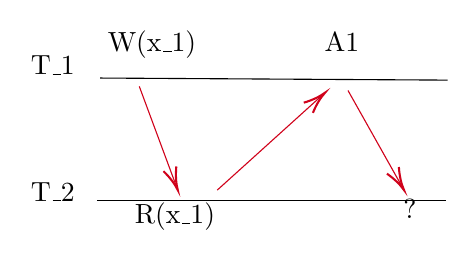
\begin{tikzpicture}[x=0.75pt,y=0.75pt,yscale=-1,xscale=1]
%uncomment if require: \path (0,300); %set diagram left start at 0, and has height of 300

%Straight Lines [id:da9500410641573396] 
\draw    (49.17,42) -- (216.56,43) ;
%Straight Lines [id:da7796185686481738] 
\draw    (47.56,101) -- (215.76,101) ;
%Straight Lines [id:da9563274467788809] 
\draw [color={rgb, 255:red, 208; green, 2; blue, 27 }  ,draw opacity=1 ]   (68,46) -- (85.86,94.13) ;
\draw [shift={(86.56,96)}, rotate = 249.64] [color={rgb, 255:red, 208; green, 2; blue, 27 }  ,draw opacity=1 ][line width=0.75]    (10.93,-3.29) .. controls (6.95,-1.4) and (3.31,-0.3) .. (0,0) .. controls (3.31,0.3) and (6.95,1.4) .. (10.93,3.29)   ;
%Straight Lines [id:da9159237520413861] 
\draw [color={rgb, 255:red, 208; green, 2; blue, 27 }  ,draw opacity=1 ]   (105.56,96) -- (156.08,50.34) ;
\draw [shift={(157.56,49)}, rotate = 137.89] [color={rgb, 255:red, 208; green, 2; blue, 27 }  ,draw opacity=1 ][line width=0.75]    (10.93,-3.29) .. controls (6.95,-1.4) and (3.31,-0.3) .. (0,0) .. controls (3.31,0.3) and (6.95,1.4) .. (10.93,3.29)   ;
%Straight Lines [id:da9009499956012581] 
\draw [color={rgb, 255:red, 208; green, 2; blue, 27 }  ,draw opacity=1 ]   (168.56,48) -- (194.58,94.26) ;
\draw [shift={(195.56,96)}, rotate = 240.64] [color={rgb, 255:red, 208; green, 2; blue, 27 }  ,draw opacity=1 ][line width=0.75]    (10.93,-3.29) .. controls (6.95,-1.4) and (3.31,-0.3) .. (0,0) .. controls (3.31,0.3) and (6.95,1.4) .. (10.93,3.29)   ;

% Text Node
\draw (14.5,30) node [anchor=north west][inner sep=0.75pt]   [align=left] {T\_1};
% Text Node
\draw (14.5,91) node [anchor=north west][inner sep=0.75pt]   [align=left] {T\_2};
% Text Node
\draw (64.56,101) node [anchor=north west][inner sep=0.75pt]   [align=left] {R(x\_1)};
% Text Node
\draw (51.56,18) node [anchor=north west][inner sep=0.75pt]   [align=left] {W(x\_1)};
% Text Node
\draw (194,99) node [anchor=north west][inner sep=0.75pt]   [align=left] {?};
% Text Node
\draw (156,19) node [anchor=north west][inner sep=0.75pt]   [align=left] {A1};


\end{tikzpicture}\\
To prevent this: If a transaction has preformed a read on a object modified by a aborted transaction, It itself has to abort.
    \item G1b: Intermediate Reads (dirty reads)
    A history exhibits G1b if it contains a committed transaction containing a read of an intermediary modification by another transaction. i.e. a read of a non final modification was preformed and committed to the history. 
\tikzset{every picture/.style={line width=0.75pt}} %set default line width to 0.75pt        

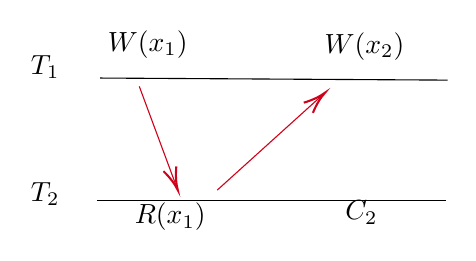
\begin{tikzpicture}[x=0.75pt,y=0.75pt,yscale=-1,xscale=1]
%uncomment if require: \path (0,300); %set diagram left start at 0, and has height of 300

%Straight Lines [id:da9500410641573396] 
\draw    (49.17,42) -- (216.56,43) ;
%Straight Lines [id:da7796185686481738] 
\draw    (47.56,101) -- (215.76,101) ;
%Straight Lines [id:da9563274467788809] 
\draw [color={rgb, 255:red, 208; green, 2; blue, 27 }  ,draw opacity=1 ]   (68,46) -- (85.86,94.13) ;
\draw [shift={(86.56,96)}, rotate = 249.64] [color={rgb, 255:red, 208; green, 2; blue, 27 }  ,draw opacity=1 ][line width=0.75]    (10.93,-3.29) .. controls (6.95,-1.4) and (3.31,-0.3) .. (0,0) .. controls (3.31,0.3) and (6.95,1.4) .. (10.93,3.29)   ;
%Straight Lines [id:da9159237520413861] 
\draw [color={rgb, 255:red, 208; green, 2; blue, 27 }  ,draw opacity=1 ]   (105.56,96) -- (156.08,50.34) ;
\draw [shift={(157.56,49)}, rotate = 137.89] [color={rgb, 255:red, 208; green, 2; blue, 27 }  ,draw opacity=1 ][line width=0.75]    (10.93,-3.29) .. controls (6.95,-1.4) and (3.31,-0.3) .. (0,0) .. controls (3.31,0.3) and (6.95,1.4) .. (10.93,3.29)   ;

% Text Node
\draw (14.5,30) node [anchor=north west][inner sep=0.75pt]   [align=left] {$T_1$};
% Text Node
\draw (14.5,91) node [anchor=north west][inner sep=0.75pt]   [align=left] {$T_2$};
% Text Node
\draw (64.56,101) node [anchor=north west][inner sep=0.75pt]   [align=left] {$R(x_1)$};
% Text Node
\draw (51.56,18) node [anchor=north west][inner sep=0.75pt]   [align=left] {$W(x_1)$};
% Text Node
\draw (166,100) node [anchor=north west][inner sep=0.75pt]   [align=left] {$C_2$};
% Text Node
\draw (156,19) node [anchor=north west][inner sep=0.75pt]   [align=left] {$W(x_2)$};


\end{tikzpicture} \\
To prevent this a: If a transaction has read a intermediate state of an object it must be aborted, or a exclusive lock should be held to prevent other transaction from accessing a intermediate state.


    \item G1c: Circular Information Flow\\
A history exhibits G1c if the DSG contains a directed cycle consisting entirely of dependency edges. There exist 3 possible combinations of such cycles: [ww,wr],[ww,ww],[wr,wr], below [wr,wr] is used for an example where T1 and T2 depends on each others writes.
\tikzset{every picture/.style={line width=0.75pt}} %set default line width to 0.75pt        

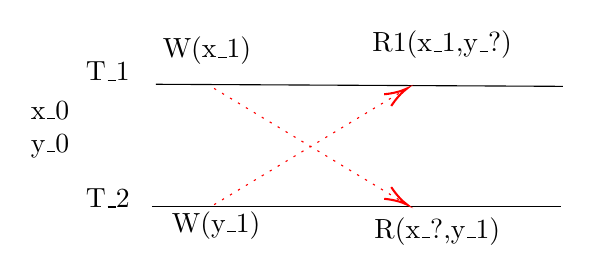
\begin{tikzpicture}[x=0.75pt,y=0.75pt,yscale=-1,xscale=1]
%uncomment if require: \path (0,300); %set diagram left start at 0, and has height of 300

%Straight Lines [id:da9500410641573396] 
\draw    (61.45,42) -- (257.56,43) ;
%Straight Lines [id:da7796185686481738] 
\draw    (59.56,101) -- (256.62,101) ;
%Straight Lines [id:da05192673528173475] 
\draw [color={rgb, 255:red, 255; green, 0; blue, 0 }  ,draw opacity=1 ] [dash pattern={on 0.84pt off 2.51pt}]  (89.56,100) -- (180.85,45.03) ;
\draw [shift={(182.56,44)}, rotate = 148.95] [color={rgb, 255:red, 255; green, 0; blue, 0 }  ,draw opacity=1 ][line width=0.75]    (10.93,-3.29) .. controls (6.95,-1.4) and (3.31,-0.3) .. (0,0) .. controls (3.31,0.3) and (6.95,1.4) .. (10.93,3.29)   ;
%Straight Lines [id:da10349511339666284] 
\draw [color={rgb, 255:red, 255; green, 0; blue, 0 }  ,draw opacity=1 ] [dash pattern={on 0.84pt off 2.51pt}]  (89.56,44) -- (180.85,98.97) ;
\draw [shift={(182.56,100)}, rotate = 211.05] [color={rgb, 255:red, 255; green, 0; blue, 0 }  ,draw opacity=1 ][line width=0.75]    (10.93,-3.29) .. controls (6.95,-1.4) and (3.31,-0.3) .. (0,0) .. controls (3.31,0.3) and (6.95,1.4) .. (10.93,3.29)   ;

% Text Node
\draw (26.5,30) node [anchor=north west][inner sep=0.75pt]   [align=left] {T\_1};
% Text Node
\draw (26.5,91) node [anchor=north west][inner sep=0.75pt]   [align=left] {T\_2};
% Text Node
\draw (165.56,105) node [anchor=north west][inner sep=0.75pt]   [align=left] {R(x\_?,y\_1)};
% Text Node
\draw (63.56,18) node [anchor=north west][inner sep=0.75pt]   [align=left] {W(x\_1)};
% Text Node
\draw (68,102) node [anchor=north west][inner sep=0.75pt]   [align=left] {W(y\_1)};
% Text Node
\draw (164.56,15) node [anchor=north west][inner sep=0.75pt]   [align=left] {R1(x\_1,y\_?)};
% Text Node
\draw (0,49) node [anchor=north west][inner sep=0.75pt]   [align=left] {x\_0\\y\_0};
\end{tikzpicture}\\
The above example has x and y in the initial state of 0, $T_1$ writes $x_1$ and $T_1$ writes $y_1$. They then read x,y. $T_1$ sees $x_1,y_0$ and $T_1$ sees $X_0,y_1$ while the actual state of the system is $x_1,y_1$
\end{itemize}

\subsection{G-cursor: Lost Update}

\todo[author=Mark]{Finish section}
\newpage

\chapter{Consistency Model testing}

\section{Introduction}
Consistency model testing is the process of testing if a given system meet the requirement for a given consistency model. The way consistency models are defined is by which anomalies they prohibit. Therefor a straight forward method for testing whether a given system meets the requirements for a model can be done by analysing the transaction history for anomalies.\\
\vspace{5mm}
The reason for doing these tests is to ensure both that a system behaves in an expected manner and to verify that they behave according to how they're presented and defined by their creators. If a system doesn't behave as expected, situations can occur where information is lost and harm can be done either bodily, financially or materially. \\ \vspace{5mm}
These situations occur as Databases often sacrifice consistency to gain performance or higher availability. In context older style transactional databases might only allow for the execution of one transaction at the time where either the whole database or tables are locked by this transaction. Other implementations allow for transactions to execute concurrently to allow for higher performance and better scalability. however it often occurs that these optimizations have side effects due to either poor implementations, understanding or simply intentionally to gain performance. These side effects might range from sometimes returning a stale value to the dirty reads and writes that allow for uncommitted data to persist 

\section{Historically}

Historically, this was done using manually defined sets of transactions. They required careful consideration and were time consuming to design, and often only able to check for simple patterns.  These tests were run on a given system checking if a proven invariant hold for a given consistency model, or if an anomaly is present in concurrent execution, This was done by inserting 2 records,  x and y in two separate transactions and in two following transactions checking if we can observe x but not y, or y and not x, as this could show how the systems handle long forks and snapshot isolation, and more importantly if it supports them at all.

These tests are generally quite efficient, but only check for certain patterns and therefore don't allow for the larger picture of where issues might be present. they are also highly limited in what they can check and which models they can check for. Furthermore due to the hard-coded and highly custom design they are implemented on a system to system basis with interchangeability is supported.

This also means that the scope of these testing projects are normally huge and defined case by case with predefined transactions that only test a limited scope. The test might have been done previously but were very limited in test coverage and most anomalies were are never detected,

\section{State of the art}

The state of the art is Jepsen, or rather one of the state of the Art projects.

The Jepsen client is build up in a modular fashion such that the different modules needed for a test can be defined independently and a given project might not require all modules. A jepsen test suite generally consist of a 5 modules. Database automation, client, generator, correctness checkers, and a fault introduce. On top of these modules a test runner is required that glues the modules together.

The goal of Jepsen was to have a framework that allows 

The more inner workings of Jepsen consist of a Host node, and tentacles going connecting to the nodes in the test cluster to preform of\todo[author=Daniela]{preform of the tasks?} the tasks such as database automation and the introduction of faults.


\section{Jepsen}
"
Jepsen is an effort to improve the safety of distributed databases, queues, consensus systems  (...) exploring particular systems' failure modes. In each analysis we explore whether the system lives up to its documentation's claims.
"\cite{jepsonio}
\\
\vspace{5mm}

Going from the above quote Jepsen is a way that allows us to check whether a given database system lives up to the requirements and premises that are given by their creators. In a world where distributed, hyper scale or even planetary scale systems are becoming the more common, this requires data storage to behave in an expected manner. The reason that expected manner is used rather than correct manner is that we may allow certain faults to occur, and allow for eventual consistency as this allows for higher throughput applications. There are case where data may only be required locally as to consider a transaction complete even in the case where some undesirable conditions occur, but these are tolerated to a certain extent. \\
\vspace{5mm}

A scenario where real time data distribution and correctness is of the utmost importance is within transactions in the finance industry, where we only want to consider a financial transaction committed once all shards of this data is replicated and the 'old' balance is no longer available. Otherwise we could reach a condition where worst case a client is able to draw a negative balance on their account or where one of the transactions isn't recorded as only one of the two transactions is recorded.\\

Oppositely a situation where eventual consistency is of no issues is for platforms like Facebook, YouTube, or Reddit. When a user comments on a post this comment might not necessary be available to users instantly and it's of no concern if it take a few seconds or minutes for it to be distributed to all nodes. Users generally don't notice these delays and it allows for better scaling within these huge applications with mullions or billions of request per second.



\subsection{Runner}

The runner is the glue that binds the underlying modules together. It contains configurations for targets, rates, how many faults should be introduced, and every other aspect of the testing suite.

\subsection{Database Automation}
 The Database or db module job is to handle starting, stopping and interaction with the database program or service itself. It's main job is to spin up, prepare and configure a test target, in some instances this might not be required but it is best practice to do this as it allows for better repeatably of the tests. A just as important feature is interacting with the service ones it is running, killing workers, inducing crashes, or removing the entire node from the cluster.

\subsection{Client}
The Client is an interface from a map of commands to a connector or driver. It handles parsing, validation of return values, exception and faults handling and routing of requests to the correct endpoint.

\subsection{Generator}
The generator's task is to generate the test map which includes transactions and faults in a manner that allow for correctness checking. in the sense that our checker needs to be able defer a ordered history from the responses from the target database.

\subsection{Correctness checker}
The checker module checks for anomalies in the results, this can be a host of symptoms, out of order operations, violation of isolation, corrupt data due to conflicts. This can either be done by writing custom checkers or by using some of the functionality built into Jepsen.

\subsection{Fault inducer}
Nemesis the the module within jepsen that induces faults, it's task is to induce faults at random such time skew, network partitions, crashes, increased package drop, increased latency and other such tools.




Jepsen supports quite a few different modules but the most powerfull features goes by the name Elle, inferring isolation anomalies from Experimental Observations. \\
\vspace{5mm}
The way this works is by inferring a dependency graph between client side observations and the database version history. This is done by carefully selecting database objects and operations such that the database reads reveals information about the version history.\\
\vspace{5mm}
This means that Elle is able to reveal any anomaly and provide a concise explanation as to why a fault occurred with information of what conditions were present to cause this fault to occur. Using this information we are able to say how a system behaves, what level of isolation and which behavior we'll see as well as what promises the system makes and how does promises are reflected in reality.\\
\vspace{5mm}

And these things can be manifested in multiple ways, some cases are, as mentioned earlier in the paper, accepted as eventually consistency and performance is valued higher or some applications where loosing some data points are acceptable to allow for higher write throughput.\\
\vspace{5mm}

And the same does for stale, dirty, non-repeatable and phantom reads aren't an issue. This could be on hyper scale social networks where if you see something that was deleted, or if the newest posts, comments and likes aren't distributed across the all notes, but they will eventually. But this is a trade off that is done to allow for much higher write performance as the chance a user is making chancing to the same page on two different nodes/clusters are minimal and the required performance drop required to facilitate the guarantee that all data is always up to date would mean that the system wouldn't scale at the rate it's required, this also brings up another interesting topic, approximate programming, where a program doesn't always have to return the correct output, but if we can see a magnitude speedup of a program and accept a faulty result rate of a few \%, then the cost saving and capacity increase could very much be worth it. This could be in the case of Netflix and Amazon recommencing products and services, it doesn't have to be perfect and maybe sometimes the result is wrong but if it means we're able to serve a lot more customers before having to degrade services or maybe having it as a step in the service degradation levels to support as many users as possible. \\
\vspace{5mm}
But a lot of this lays outside the scope of this thesis but it's also a super interesting field that will probably see grow in the next decade.


\subsection{Elle}


The way this works is by inferring a dependency graph between client side observations and the database version history. This is done by carefully selecting database objects and operations such that the database reads reveals information about the version history.\\
\vspace{5mm}
This means that Elle is able to reveal any anomaly and provide a concise explanation as to why a fault occurred with information of what conditions were present to cause this fault to occur. Using this information we are able to say how a system behaves, what level of isolation and which behavior we'll see as well as what promises the system makes and how does promises are reflected in reality.\\

\todo[author=Mark]{Finish Subsection on Elle}
Elle is a consistency checker and generator available in Jepsen. It supports a few different methods 
\\
Elle is the one of the Jepsen Consistency checkers available in jepsen, other exist but for all intents and purposes Elle should always to used. 
Introduction to Elle
... \\
What it aims to solve
...\\

...\\
Checker
...\\
Generators
...\\
TXN
...\\

% move these to BIB file and write this section
% K. Kingsbury. Knossos.
% https://github.com/jepsen-io/knossos, 2013-2019.

% G. Lowe. Testing and Verifying Concurrent Objects.
% Concurrency and Computation: Practice and
% Experience, 29(4), 2017

% J. M. Wing and C. Gong. Testing and Verifying
% Concurrent Objects. Journal of Parallel and
% Distributed Computing, 17(1-2), 1993.

% P. B. Gibbons and E. Korach. Testing shared
% memories. SIAM Journal on Computing, 26(4), 1997

% S. Burckhardt, C. Dern, M. Musuvathi, and R. Tan.
% Line-up: A Complete and Automatic Linearizability
% Checker. PLDI '10, 2010.





\section{Past Jepsen tests}
    Finding in past Jepsen test.
\subsection{Cassandra}
A test was done on Cassandra in 2013 that showed some interesting behavior, with interesting names such as doomstones, and that doing conflicts a lexicographically bigger value is winning. such that separate parts of separate transactions might end up in the database. .\\
\vspace{5mm}
Casandra itself is built on a hash ring via a distributed hash table like Service Fabric. but unlike most other database it uses timestamp based last write wins. This allows for extremely high performance but also at the cost of being highly sensitive to clock skew.\\

In the test on Cassandra it was found that:
\begin{itemize}
    \item doing a single key heavy write operations Losing 28\% of committed data and fails linearizable by any definition.
    \item Doing Write conflicts roughly 1 in 200 rows end up being corrupt due to poor handling time time where milliseconds are used with 3 zeros at the end instead of microseconds.
    \item \textit{No. Cassandra lightweight transactions are not even close to correct. Depending on throughput, they may drop anywhere from 1-5\% of acknowledged writes–and this doesn’t even require a network partition to demonstrate. It’s just a broken implementation of Paxos. In addition to the deadlock bug, these Jepsen tests revealed \#6012 (Cassandra may accept multiple proposals for a single Paxos round) and \#6013 where an insert is rejected but committed anyway. (unnecessarily high false negative probabilities).}
\end{itemize}

https://aphyr.com/posts/294-call-me-maybe-cassandra


\subsection{Postgres}

\begin{itemize}
    \item \textit{Users should be aware that PostgreSQL’s “repeatable read” is in fact snapshot isolation — a fact long-understood in the PostgreSQL community and previously reported by Kleppmann. Since G2-item is prohibited under common formalizations of repeatable read, users may have designed applications assuming this held true for PostgreSQL. In this case, users may wish to run selected transactions under serializable isolation instead, add explicit locking, or redesign those transactions such that they are no longer sensitive to G2-item.}
    \item \textit{It appears that no version of PostgreSQL has ever guaranteed serializability. Users should be aware that concurrent update and insert transactions may exhibit G2-item. High-contention workloads are especially susceptible. The PostgreSQL team has written tests to reproduce the problem and is evaluating a patch; we recommend upgrading once the next minor release becomes available.}
\end{itemize}
https://jepsen.io/analyses/postgresql-12.3

\section{related work to Jepsen}

\todo[author=Mark]{ move these to BIB file and write this section}
% K. Kingsbury. Knossos.
% https://github.com/jepsen-io/knossos, 2013-2019.

% G. Lowe. Testing and Verifying Concurrent Objects.
% Concurrency and Computation: Practice and
% Experience, 29(4), 2017

% J. M. Wing and C. Gong. Testing and Verifying
% Concurrent Objects. Journal of Parallel and
% Distributed Computing, 17(1-2), 1993.

% P. B. Gibbons and E. Korach. Testing shared
% memories. SIAM Journal on Computing, 26(4), 1997

% S. Burckhardt, C. Dern, M. Musuvathi, and R. Tan.
% Line-up: A Complete and Automatic Linearizability
% Checker. PLDI '10, 2010.




    \newpage


    \chapter{Modern Datastores}

    The thesis will primacy focus on Service Fabrics but investigation into other data stores is also done to allow comparisons and investigation into what different models affect the behavior of the database systems.


    \section{Service Fabric}

%    https://www.microsoft.com/en-us/research/wp-content/uploads/2016/02/tr-95-51.pdf
%
%    https://docs.microsoft.com/en-us/azure/service-fabric/service-fabric-reliable-services-reliable-collections

    \subsection{Introduction}

    Service Fabric (SF) is presented as a distributed systems platform something akin to Kubernetes (K8S), where the user is able to build, deploy and scale micro services and containers. One of the key points presented by Microsoft on Azure Service Fabric is that you're able to run stateful services. It's presented by Microsoft as the backbone of their core services and data stores.\\
    \vspace{5mm}

    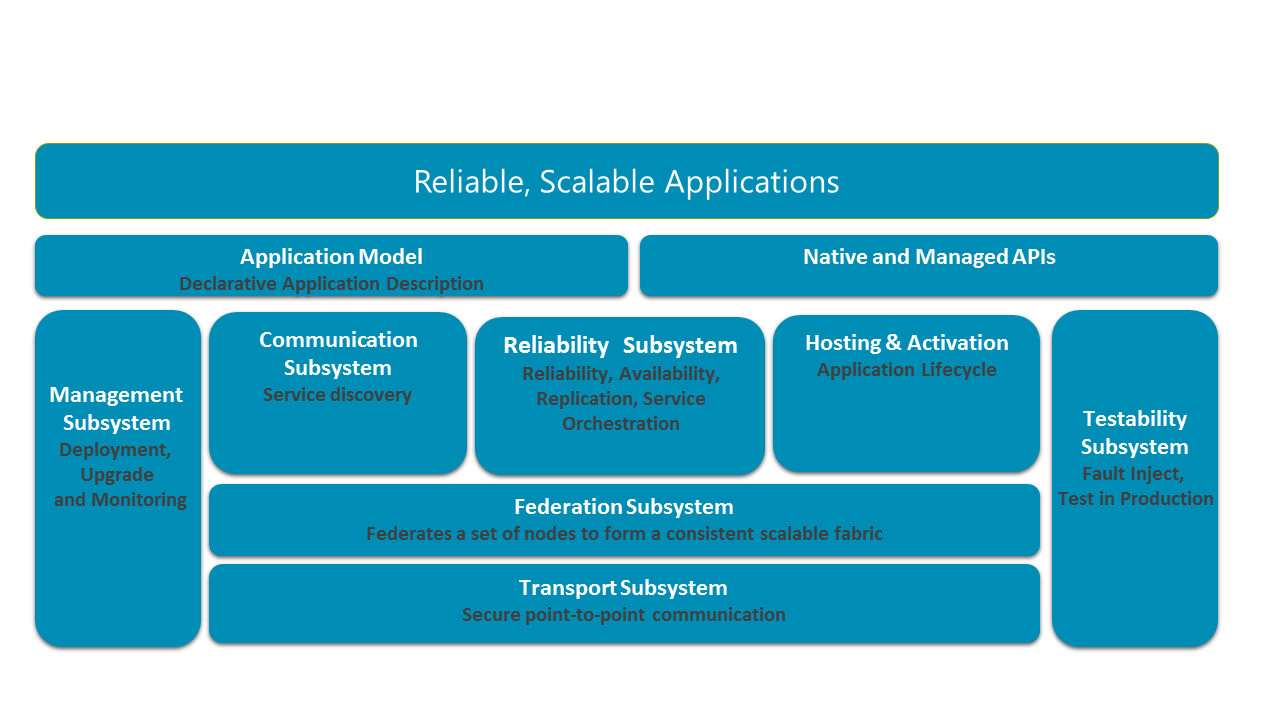
\includegraphics[scale=0.5]{images/service-fabric-architecture.png}

    \subsection{System Architecture}

    The architecture behind Service Fabric is built via a layered approach, by Microsoft's words this allows developers to write applications that are highly available, scalable, manageable and testable. These layers are built on 5 Core and 2 supporting subsystems. Our main interest lies within the reliable collection so I will only be investigating the layers and services that lay below this.\\
    \vspace{5mm}

    \subsubsection{Transport subsystem}
    \todo[author=Mark]{these might be serving the same purpose and the documentation might just be odd.}
    The lowest layer in the core stack that provides secure communication within the cluster itself and between the cluster and clients. This functionality is provided via point to point communication channels that support one way and request reply patterns, in other terms UDP and TCP. This also provides basis for broadcast and multicast within the cluster. Security is handled via wither windows security or x509 certificates. \\
    \vspace{5mm}

    \subsubsection{Federation subsystem}

    The next subsystem in the stack is the Federation subsystem, this uses communication channels provided to it by the transport subsystem to gather the nodes into a unified service fabric cluster. It also provides system primitives that allow for Failure detection, leader Election and consistent routing within the cluster by upper layers in the system.\\
    \vspace{5mm}

    The core of the subsystem is built around an SF-ring that was developed internally at Microsoft in the early 2000s, where both keys and nodes are mapped to a point in the ring, with keys being owned by the node closest to it in the ring. Each node also uses this ring to keep track of its immediate successor and predecessor nodes that it stores in a Neighborhood set, this set is then used by the Federation layer to run consistent membership and failure detection. Nodes also maintain long distance routing partners that are used for consistent routing.\\
    \vspace{5mm}

    The membership and Failure detection is done using tow key design principles.\\
    \vspace{5mm}

    Strongly Consistent membership and Decoupling Failure Detection from Failure Decision\\
    \vspace{5mm}

    \begin{itemize}
        \item \textbf{Strongly Consistent membership} All nodes monitoring a given nodes status must agree on weather the node is up or down. For use in the SF ring this means that the all nodes on the node's Neighborhood set must agree on its status.
        \item \textbf{Decoupling Failure Detection from Failure Decision}: Failure detection protocols can lead to conflicting states, therefore the decision is decoupled from detection.
    \end{itemize}
    \vspace{5mm}

    To solve the issue of decoupling failure detection and the decision making on these failure, all decisions is distributed to a set responsible nodes. This Ensures that decisions are performed in a consistent and reliable manner. The detection of failures is performed via a distributed monitoring and leasing solution implemented in SF. This implementation solves this via Lease Renewal Request(LR) and LRack(Lease Renewal Acknowledgement). A node is simply required to maintain valid leases from all of its monitors and these leases have to be renewed every lease period. This leasing period is calculated based on round trip times within the cluster. If a node fails to renew any of these leases it considers removing itself from the set of nodes. If a monitor misses a lease request to a node, the node turn considers marking the monitor as failed. Both of these decisions need to be approved by an Arbitrator group. If a node fails to receive an LRack within a timeout based on round trip time, it repeats the LR until it receives an LRack. Due to the nature of the SF-ring these monitor relations are symmetrical, but this Lease protocol is still run independently, there are however other cases. If a node fails the renewal process, it stops renewing leases to any other nodes, or if a node detects another node as having failed, it stops sending renewal request to it. These 2 cases have the potential to cause inconsistencies if they were operating alone, however decision of deciding if a node is down or up is up to the Arbitrator group, which maintains consistent memberships. \\
    \vspace{5mm}

    The decision to determine failures is preformed by the Arbitrator group. This is separate from the neighborhood set. They operate independently and it has two ways of deciding if a given node has failed. The way that the groups stay consistent when members join or leave the group is that when an Arbitrator joins the set, it initially rejects all requests in the first T seconds. This is done to prevent new Arbitrator making conflicting decisions with the excising nodes, and to prevent failed nodes to exist in the distributed membership protocol. This ensures that detected nodes leave before being forgotten.\\
    \vspace{5mm}

    \begin{enumerate}
        \item X detects Y as failed and sends fail(Y) to the arbitrator
        \item The arbitrator adds Y to a recently failed list and sends ack(fail(y)) containing a timeout for Y to X. If The arbitrator already marked X as having failed and ignores the request,
        \item If X receives this request it waits for the TO to claim Y's area of the ring. and if re receives no response within the timeout it leaves itself.
    \end{enumerate}

    If a node is already in the recently failed list, it returns the same response as to the first reporter except it calculates the time since first detection so the portion of the ring it own is claimed by the neighbors at the same time. This also means that the routing can continue after Time out with a laxity added. As all routing request for a node are added to a queue if a node is marked as failed. The queue is then released after Timeout+laxity that allows all neighboring nodes to claim that part of the ring and allows to these routing request to be preformed by its successors.\\
    \vspace{5mm}

    If the case of two nodes reporting each other as failed, the conflict is resolved either by majority. The node that was reported first to the most Arbitrators leaves the ring. A second option is to heal the membership if both nodes are healthy and can therefor be allowed to stay. \\   \vspace{5mm}
    
    The implementation in SF is presented as being failure tolerant towards cascade failures as the decision isn't made by the detectors themselves but by arbitrators.
    This can be in cases of network congestion or partitions that result in multiple nodes detecting each other as failed. where traditional distributed hash tables this can result in inconsistencies in the membership lists or ring.\\ 
    \vspace{5mm}

    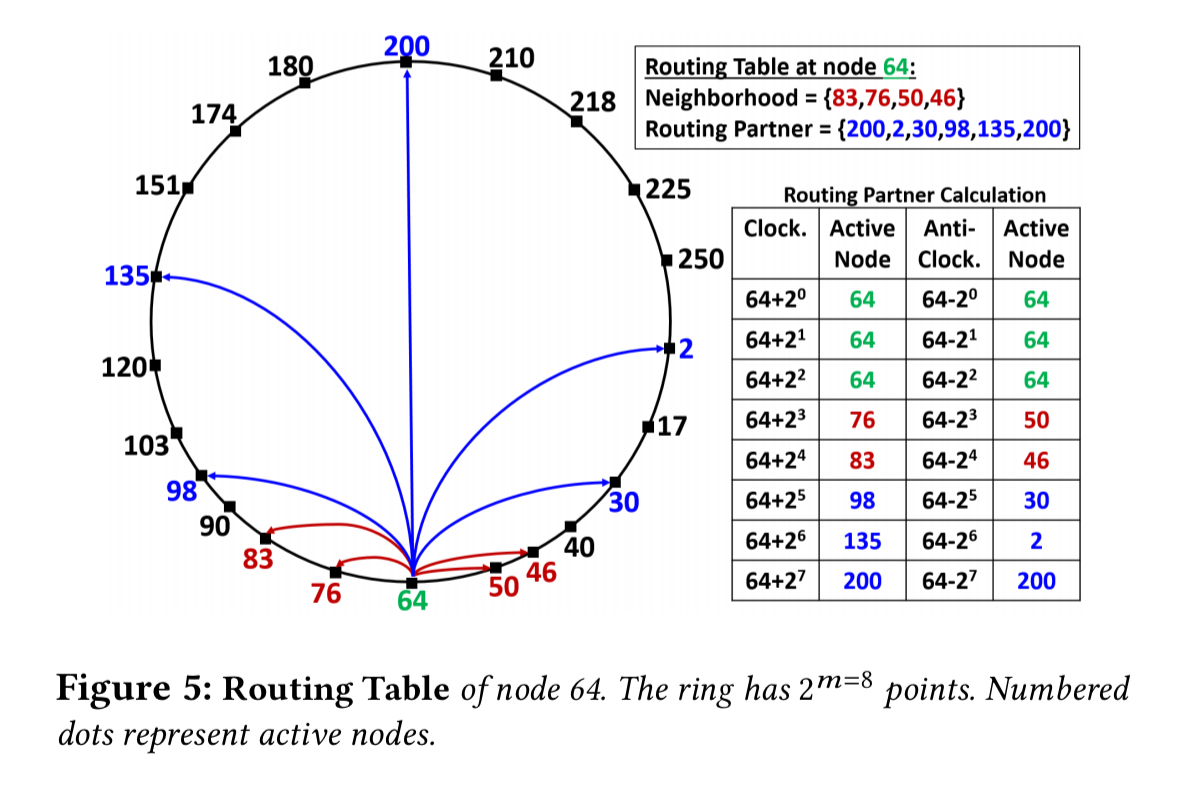
\includegraphics[scale=0.3]{images/servicefabric-fig-ring-topology.jpeg}

    SF-Ring and consistent routing.(need to rewrite/reword this to a more coherent sentence.)

    The Distributed Hash table used for service fabric routing is a evolution of SF-ring that was developed within Microsoft in the 2000s. The routing used offers symmetry and due to this it allows bidirectional routing that allow for lookup and routing via binary search. This allows SF to route message around the ring in a fast manner, with multiple routing options in that there always exist 2 routing partners on either side of the destination that both helps distribute the load and is able to route even with stale routing tables. Initially all packages were routed using this method, this has changed over the years. Today the hash table is used to build a routing table and maintain it when a new node is added to the cluster. After discovery a direct route is used via the destination IP address. \\
    \vspace{5mm}

    Routing tables work differently depending on the size of the cluster. However it is able to route in two ways. If the size of the routing table is smaller than the number of nodes a direct route is used, if there exist more nodes in the cluster than the routing tables it switches to routing via routing tables to reduce memory consummation but causing an increase in time complexity to O(Log(n)) from O(1)\\
    \vspace{5mm}

    Routing Tokens.
    \todo[author=Mark]{I was unable to find information on this precisely is handled however from the wording in the paper the initially split would be 50/50 and a third node would be 50/25/25? is it split evening it 33/33/33 but a Fourth node would be 22/22/22/33 that would cause unbalance unless some shifting is done}
    Each node owns a token that includes a portion of the routing token it is responsible for. The SF-ring protocol ensures two properties:
    \begin{itemize}
        \item Each token is only owned by one node at any given time;
        \item Eventually every token is owned by 1 node.
    \end{itemize}
    This ensures SF handles nodes joining and leaving the ring. Initially a bootstrap node owns the entire ring. After the initial bootstrap node, any joining node will split the ring segment between them. Routing tokens are also used for leader election, simply the owner of a given key is the owner. This same process ensures no keys are abandoned.

    \subsubsection{Reliability subsystem}
    The reliability subsystem is in charge of load balancing, replication and availability. These three aspects are provided via 3 services: a Failover Manage, a Naming and Resolution, and a Placement and lastly a Load Balancer service.\\
    \vspace{5mm}

    The Failover Manager is running as a stateful service, that has an instance running on each node in the cluster, that provides 3 actions: start a replica, move a replica, reconfiguration of a replica.\\
    \vspace{5mm}

    \begin{itemize}
        \item \textbf{Create a replica} Create a new replica when instructed by the PLB
        \item \textbf{Move a replica} migrate a replica when instructed by the PLB to a different node.
        \item \textbf{Reconfiguration} If a primary replica becomes unavailable, promote a secondary as the new primary, in case the old primary comes back only it is demoted to secondary.
    \end{itemize}

    A service called Failover Master Manager is also running that is able to restart the failure manager via a cached state in case it fails. In case the master fails it is able to rebuilt its state via the SF-ring. The Master Failover manager is running on the node who's token range contains ID0.\\
    \vspace{5mm}

    The naming and resolution service maps instance names to endpoints that services are listening on. This allows for consistent routing from outside of the cluster via URI that doesn't change over their lifetimes.\\
    \vspace{5mm}

    The Placement and Load Balancer(PLB) service is stateful and is in charge of placing replicas and instances of services on nodes and ensures an even load throughout the cluster. They claim that unlike other solutions where services are hashed onto the ring in SF, the PLB explicitly assigns each service replica Primary and Secondary nodes in the Ring. It continually monitor the cluster for available resources. This allows for assignment and migration of services to underutilized nodes,  more importantly it ensures services are migrated away from a node that is about to enter a service window or in cases of over-utilization that could lead to service degradation\\
    \vspace{5mm}

    The technique used for selecting placement of nodes is done via Simulated Annealing, as it is presented to provide a near optimal solution as to where services can be placed. The way the system is modeled is via resource use in the system where an even load is desired, but some constraints need to be met such as fault tolerance, avoiding replica co-location and some service might have a strict set of nodes to run on. \\
    \vspace{5mm}

    \subsubsection{Reliable Collections}

    Reliable collections provide stateful services in Service Fabric via Reliable Directories and Reliable Queues that are available for C\# and Java programming, and are promised to be:
    \begin{itemize}
        \item Available and Fault-tolerant via replication,
        \item Persistent via disk
        \item Efficient via asynchronous via API that are non blocking.
        \item Transnational via APIs with ACID semantics.
    \end{itemize}

    One of the key differences between storage systems built on SF and other highly-available systems is that states are kept locally in the replica while also being made highly-available. This causes most reads to be local.\\
    \vspace{5mm}

    Writes are relayed from the primary replica to secondary replicas via passive replication. A write is considered complete when the majority of secondaries acknowledge it. The relaxations allow an application to achieve weaker consistency by relaxing where a read can go, eg: always read from primary to read from secondary. \\
    \vspace{5mm}

    SF is presented as the only "self-sufficient microservice system that can be used to build a transactional consistent database which is reliable, available, self-*, and upgradeble because the lower layers assure consistency"\cite{SFpaper} \\
    \vspace{5mm}

    \paragraph{Consistency models/isolation levels}
    SF reliable collections promise two Select-able consistency models that the user can pick. Repeatable Read and Snapshot Isolation. eg there is no promise about Serializability of the transactions.\\
    \vspace{5mm}

    \begin{table}[h]
        \centering
        \begin{tabular}{l|l|l}
            & \multicolumn{2}{c@{}}{\text{Role}} \\
            \text{Operation}   & Primary         & Secondary \\
            Single Entity Read & Repeatable Read & Snapshot  \\
            Enumeration, Count & Snapshot        & Snapshot
        \end{tabular}
        \caption{isolation level defaults for Reliable Dictionary and Queue operations.}
        \cite{SF_RC_Transactions}
    \end{table}


    \section{Programming for Service Fabric}
    
    Development for the Service Fabric Framework is done closely resembles the Development flow for Dotnet Web applications and Kubernetes service Development, There are however tighter constraints where the application is only executable in azure as no local development environment exist for Linux. \\
    
    Writing the code itself is possible via either Java or C\#. Documentation only really exist for C\#, however this documentation also seem to be outdated and lack quite a bit of information. Generally a MVC application is the best choice for architecture of the service itself where stateless or stateful variants are available.\\
    
    Debugging and testing code on the Linux implementation is highly lacking with no debug tooling available such as remote executing with a debugger or support for dump files to analyse crashes and issues within the application. This caused development to be slow paced, trail\&error and draining. i would recommend creating a working application, prior to integrating the Service Fabric functionality. On top of this using heavy logging from the application to an external store that allows for insight.
   \\
   A careful note here should also be taken as there isn't features parity between platforms which causes core functionality to be unavailable on Linux.



    \section{Comparison}
    In many of the papers published by Microsoft a lot of comparisons are made to Cassadra, Redis and Dynamo. Therefore, a introduction will be made to two of these as they are comparable in a lot of aspects. The investigation won't be as deep as with SF but a investigation of consistency and failure modes will be be done.
    
    
    
    \subsection{Cassandra}
\todo[author=Mark]{Finish subsection}
    Facebook database product made opensource,
    
    Ring via hash table
    
    Last write wins
    
    Leaderless
    
    scalability
    
    Clock skrew issues
    
    Handling of conflicts
    
    sensitivity to time desync
    
    possible solution ?
    
    usecases
    
    

    \subsection{Redis}
\todo[author=Mark]{write section on Redis}

    \subsection{Dynamo}
\todo[author=Mark]{write section on Dynamo}


    \section{Comparison}
\todo[author=Mark]{write Comparison between the 3 datastores}
    In many of the papers published by Microsoft a lot of comparisons are made to Cassadra, Redis and Redis. Therefore, comparisons will be made to these as they are comparable in a lot of aspects. The investigation won't be as deep as with SF but investigation of consistency and failure modes will be be done.


    \chapter{Jepsen Test on Service Fabric Reliable collections}


    One of the goals of the thesis was to attempt to perform a Jepsen test on Service Fabric Reliable Collections subsystem. Reliable Collections powers services in Azure and is the target of this endeavor. 
    In this chapter we will present the design, implementation and revisions of the testing suite. \\
    \vspace{5mm}
    To perform such a test we need to build up both a testing suite, APIs and libraries to allow for a connection between the Jepsen service and the Service Fabric core components. Therefore, a few different applications and services need to be learnt, understood, designed, implemented, tested, executed, and at last the data generated from this can be analyzed.
    
    
   
    \section{Design \& implementation}
    The Design of the services required for preforming the Jepsen test were revised multiple times following a a learn by doing methodology as I did have no prior experience with Service Fabric, Jepsen, C\# or Clojure. 

    \subsection{Initial Design}

    The initial design of the of the testing suite contained two applications. The first one is a Service Fabric application containing a stateful and a stateless Service. The second application is a Clojure application running the Jepsen testing suite.

    \subsubsection{Service Fabric Services}

    The Service Fabric stateless service contains operation our Jepsen test can interact with. These should then be routed to the correct stateful service partition. The initial design contained endpoints for insert, add, Update, Check\&set, delete and delete all, which operated on a reliable directory datatype. The service is implemented using C\# as the lack of documentation for Service Fabric for Java made this this seem as the better choice (as of writing, nearly all this documentation is for the C\# language). Both services will expose these endpoints via the Kestrel web server. This was made as it is the native implementation already integrated into SF, had the most documentation and was therefore deemed the safest choice to proceed with.\\
    \vspace{5mm}
    A flow diagram for the design of the stateful service contains the following functionality. The Stateless service simply works as a forwarding service as is simply a 1:1 mapping with partition calculations for use in routing of the request. \\
    \vspace{5mm}
    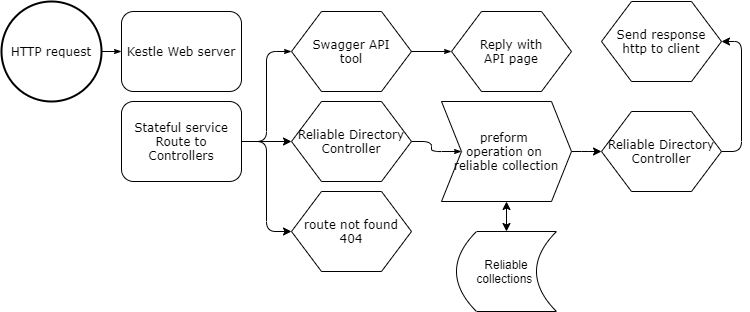
\includegraphics[scale=0.5]{images/Design_Stateful_service_1.0.drawio.png}
    \todo[author=Jacopo]{missing description of this figure. What are these components? Time allowing provide some text explaining what this figure is suppose to say}

    This implementation contains 2 main codebases. The C\# dotnet web services that acts as a API to the reliable collections using 3 controllers for the 3 default data structures implemented in the framework, and a Clojure codebase containing the Jepsen test and a driver for connecting to the Service fabric services.

    \subsection{Infrastructure}
    The infrastructure is centered around Azure, using an isolated v-net containing 6 virtual machines all running Linux. Ubuntu was chosen as it's a known distribution that we are familiar with. 1 of the 6 nodes is running the Jepsen application while the 5 remaining notes are running the Service Fabric Cluster.
    The 5 Service Fabric nodes are mostly self managing.\todo[author=Jacopo]{what does it mean mostly self managing?} Applications can be deployed via either the Azure Service Fabric CLI \cite{servicefabriccli} or via Visual Studio \cite{servicefabricguide}. The latter was the process used during the development stages of the project.

    The Jepsen host is manged and accessed via ssh. For deployment a deployment pipeline was considered but was decided against due to development overhead. A solution using scp was chosen instead due to the quicker development cycles and the fact that only a single machine required access to the deployment. 
    

    The topology of the network is arranged such that the 6 nodes are located in the same VLAN to keep connections local and prevent outside connection from causing issues with the test.\\
    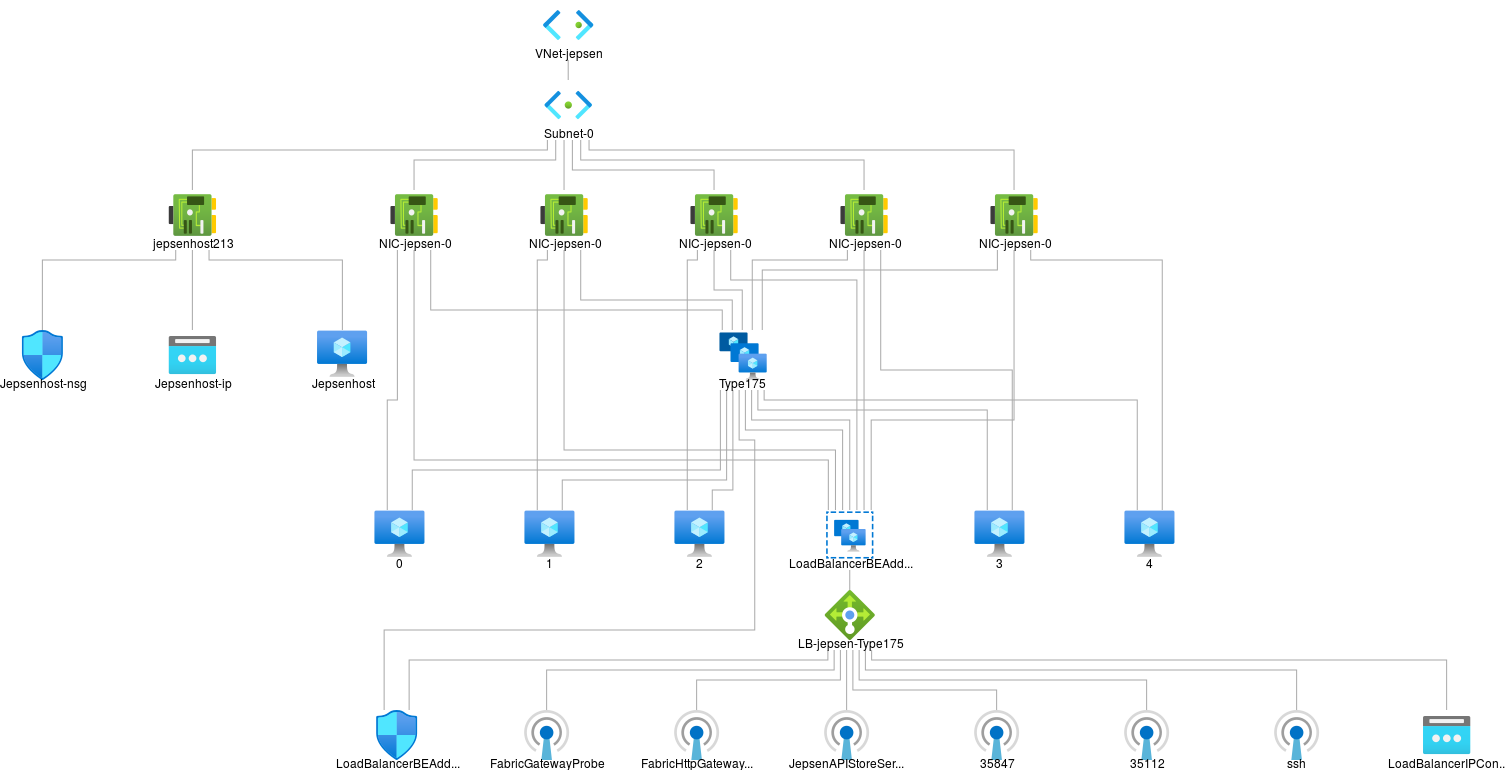
\includegraphics[scale=0.3]{images/topology.png}
    \\
    \todo[author=Jacopo]{missing description of this figure. What are these components? Time allowing provide some text explaining what this figure is suppose to say}

    All traffic resides within the cluster. The load balancer is part of the standard service fabric deployment and allows for connection to management interface, deployments and access to the underlying hosts. These endpoints were protected by firewall rules that only allowed connections from approved sources to avoid external influence of the results.

    \subsubsection*{Node Sizes}

    The initial node size contained 2vcpu, 8 GBs of ram and 20 GB local storage, as this was thought be enough to handle the workload of the test. This was later revised as the nodes had issues with disk space and often took a long time to setup and get ready for any given deployment. This problem was resolved by upgrading the size of the nodes to 4vcpu, 16GB ram and 80GB local storage per node. This configuration resulted in a more well-behaved cluster. This node size was kept for the reminder of the project. However, the Jepsenhost is slightly under-dimensioned compared to the workload it handles when computing on the result of the test. This is primary due to out of memory errors that could be solved by lowering the search space of the test or increasing the memory of the node itself.


    \subsection{Services}
    As mentioned earlier, running these tests required multiple components. The stateful service that hosts the reliable collections from SF Reliability subsystem, a stateless front-end that provides this data to clients via an API, a driver that handles the connection to this API and finally the Jepsen test suite itself consisting of workloads, generator, checker and Nemesis module..

    \subsubsection{SF services}
    Microsoft recommends using two services, such that a Statefull service is never directly exposed to the internet but where a stateless services acts a proxy. This provides multiple benefits but also a few negatives. The prime benefit is abstracting from the back-end and adding a layer of validation, routing, and protection of the back-end service. Time connections are held open should also be reduced to due round trips times being lower, which should allow for higher throughout.

    \paragraph*{Stateful Reliable collection service}

    The stateful services provides 3 separate controllers that each expose one of the built in reliable collection data types, These 3 being: Reliable Dictionary, Reliable Queue, and Reliable Concurrent Queue. Faults are also handled at this stage where faults caused by transactional issues are returned to the client via http status codes\cite{wikihttpstatuscodes}: node not primary, accepted, result not found, etc. This should allow for easier diagnoses and handling of faults when they are parsed by the Clojure application.

    The fronted stateless service simply provides these same APIs but with wrappers and routing in case of a portioned design. This layer could also be used to build additional features, but this was not the case as only the bare transactions supported by the reliable collections layer was needed.

    \paragraph*{Jepsen test suite}
    
    The design of the Jepsen test suite aims to use skeleton code from a past Jepsen test to start the project as it gives a template of what functionality should be implemented. These implementations are still custom but it gives a pointer to what the bare minimum is to have a functioning application.
    \\
    The first module is a Driver that allows our test to connect to our stateless API. Options here are to either write it in Java or Clojure. An attempt will be made to implement this in Java but depending on implementation issues or compatibility issues Clojure might be the choice. This module should handle connections, exceptions, and parse values in both directions.\todo[author=Jacopo]{did you use Java or Clojure. Here write the final result, not speculation.}
    \\
    The Jepsen suite should use a modular setup that allows interoperability between multiple workloads, a runner that allows for test tuning, db that deploys, configures and operates on the running datastore, a client runs the transactions via the driver, nemesis that induces faults in the cluster and 3 workloads, queue, concurrent queue, and dictionary. One workload for each of the transactional data types exposed by Service Fabric.
    \begin{itemize}
        \item The runner module is the main class and handles defaults, CLI input and workload selection along with configuration of common behavior shared between workloads, nemesis, db, along with other features that are mutual for all workloads.
        \item   The db module should handle spinning up and tearing down the services along with functions for stating, stopping, and killing services and workers in the cluster.

  \item  The nemesis modules should contain the functions that kill, partition or in other ways introduce failures in the cluster.

  \item 3 Workers, that act on different data types and each requiring a separate generator, checker and client.
    \end{itemize}
    
    Of the 3 workloads designed only one should be used for the final testing as they should all exhibit the same symptoms if issues exists, but all 3 are initially implemented as to allow for deciding on which type should be focused on.
    

  

\subsubsection{Implementation of the initial design}

The initial design targeted the reliable collection dictionary datatype. It presented a few issues with the design and implementational details that were not considered. The biggest obstacles when developing for Service Fabric the non feature parity between Linux and the windows implementation, this is caused by two parallel implementations where some core functionality isn't yet available in the Linux implementation. This resulted in unfavorable conditions with no debugging support, dump files that weren't readable, lack of documentation and black box behavior as local code execution wasn't possible. \\ \vspace{5mm}
A large amount of time was spent debugging, changing configuration files, stripping any unneeded libraries and rolling back to older versions of frameworks used. It should be noted that the Service Fabric framework was kept at the same release while .NET and similar aspects where rolled back to older releases.

All of these attempts were however frugal, after spending newly 2 months deleting all code, restarting from scratch using a different approach. An attempt at the implementations via Java, which was also unsuccessful, and finally going back to C\#. After getting a working solution of the project on a Service Fabric Cluster running on a windows host, i reached out to Mikkel Hegnhøj from Microsoft for assistance.

The issue turned out to be 2 fold.
\begin{itemize}
    \item .NET needing to be rolled back to 3.5
    \item The entry point having to be defined via .NET and the name of the DLL file. This was something I attempted prior by using an entry point via a bash script, as documented in the official doc. 
\end{itemize}

Finally I had a working version on Linux, or rather, I had a way to run my application on Linux as the issues didn't stop here. The Feature parity was still there. The DNS routing service is missing from the Linux implementation, this required endpoints to be hard coded, where each service was bound to a given port. This introduced a limit of 1 replica of a given service per node. This greatly reduce horizontal scaling as we need an extra node per partition. Running larger partitions on each node is also an option, but from a performance, availability, and reliability perspective it's much more effective having lots of smaller partitions, instead of one large database instance that introduces higher risks of deadlocking and along with other issues.


\paragraph*{Implementation details SF}

The design uses 2 service: a  stateless service that processes the the incoming request and routes it to the back-end service. The get key endpoint will be used to outline the design. All the stateless endpoints closely resemble each other, therefore only this will be included here.\\
        
\paragraph*{Stateless Service}
The Stateless service is implemented via Model View Controllers (MVC) that expose the website via a kestrel web server. Each endpoint route is defined via flags which define protocol and request type followed by paths and an endpoint name. A http get request using a path variable as a parameter, The \textbf{"[HttpGet("{key}")]"} flag is used. This is then followed by a function that allows the MVC design pattern, but this function a Async function that takes the key as a variable and returns a \textbf{"Task<IActionResult>"}. The used return type allows for the return value to be either JSON or predefined methods to return bad request, No Content, or other http response codes without requiring explicit handling of them.
\begin{lstlisting}[language=csh]
public async Task<IActionResult> Get(string key)
\end{lstlisting}   

The underlying Service Fabric framework exposes an endpoint that is used to retrieve all partitions of given stateful service. This is coupled with the internal routing in the transport subsystem, such that any service in the cluster can easily and securely be found and reached. 
\begin{lstlisting}[language=csh]
    ServicePartitionList partitions = await this.fabricClient.QueryManager.GetPartitionListAsync(serviceName);
\end{lstlisting}   
This allows us to query the individual partitions, where any aggregate operations are handled in the stateless service.
\begin{lstlisting}[language=csh]
    foreach (Partition partition in partitions)    {  .. Do something ..  }
    return result;
\end{lstlisting}  
\paragraph*{Stateful Service}

The stateful service was implemented via the MVC patterns as well and followed a design that kept simplicity in mind where each endpoint exposed and preformed one operation and committed this change to the datastore. This allowed for querying the database in a quick and consistent manner even if data split among  partitions.
\begin{lstlisting}[language=csh]
        [HttpGet("{key}")]
        public async Task<IActionResult> Get(string key){
        ...
         while (await enumerator.MoveNextAsync(ct)){
                  if (enumerator.Current.Key == key)
                  { return this.Json(;(enumerator.Current);
    }}}
\end{lstlisting}   

\paragraph*{Implementation details Clojure}
 
 Doing the initial implementation of the jepsen test, quite a few aspect of the program were rather chaotic. Poor programming practices that don't carry well over from object oriented  programming, into dynamic and functional programming. The Clojure programming language was treated as a learn by doing. This resulted in the first implementation of the application functioning, but not without issues. most of these were a cause of not fully understanding the language i was using and how the information flow was handled. this caused issues with HTTP requests being handled incorrectly and responses not being parsed correctly into the history such that transactions with a status of failed were considered valid in the history used to check the consistency of the model.
 
 This caused the whole application to exhibit a broad range of unintended and weird behavior, resulted from asynchronous distributed systems being complex and concurrent applications handling 100s, or 1000s of threads requiring careful planning and considerations.
        
        
The Clojure application itself is split into different modules that expose and classes. the core modules required to make up a jepsen test suite requires a runner, generator, nemesis(a type of Chaos monkey)\cite{Choasmonkey}, db, client, connector/driver and workloads.
\begin{itemize}
    \item The \textbf{Runner} contains the the majority of the configurations and a CLI interface that exposes options and settings where generalized values for the tests are specified. This is also where a select Workload is chosen for running the test. in total 3 different workloads were implemented that each require a generator, checker, client, and Nemesis.
        
   \item  The \textbf{Generator} class generate a list of transaction to execute, which can later be used to check the transaction history for any anomalies. this is closely linked with the checker.
        
   \item  The \textbf{checker} checks for anomalies in the transaction history, This could be by either checking if all committed values exist in the data store after the test, if there are transactional violation in the data store, if odd behavior like the case of Casandra where multiples objects are merged due to conflicts that might lead to unintended outcome. 
        
  \item  the \textbf{client} interface maps Jepsen operations to a connector or driver calls for a given data store. This module processes the map generated by our generator into transactions, parses the transaction into a format the driver understands and back into a format jepsen understands as well as handling any errors, exception as well as basic check if the operation failed and succeeded and logs this to the internal transaction history handled by jepsen.
\end{itemize}
        
The Jepsen application required a driver to be written for jepsen to be able to interact with the API exposed by the stateless service, This could have been written in either java or Clojure. An attempt was made to implement this in Java with some success but was scrapped and a implementation was done in Clojure instead. The Driver preforms http/https calls to the service fabric cluster and handles some input validation as well as connection management, fault handing of connection, as well as parsing of any faults and results returned by the service into a format compatible with Clojure.
        

\subsubsection{Resolving issues with the design.}
    

The initial version of the service fabric has some issues with the stateless service where the connection buffer simply overflew due to a high number of connections from the jepsen host, which caused issues for connections between the stateless service and the underlying state full services that provided the data.

A few considerations on how this issue could be resolved was considered, lowering the latency between nodes in the cluster, removing the stateless layer and connect directly to the state full service. A choice here was made to scrap the initial implementation for Service Fabric and redesign it to only require a stateful service. The transactions would behave the same in a  single partition compared to a cluster with 500 partitions, as each "master" node will behave the same, either way with the implementation that service fabric exposes. The service should therefor have a master node as well as a few active replicas that allow for checking of replication status if this should be required down the line. this resolves and simplifies two things. Routing to the separate partitions is no longer an issue as the stateless "proxy" node is removed, we no longer need to consider routing data to the correct node from our Clojure connector, where it's possible to route all traffic to the primary or only route writes to the primary while distributing the reads to check for replication issues. This allows for testing of the replication engine in the future.

 \subsubsection{Implementation of the revised design}

The implementation of this \todo[author=Jacopo]{I lost it. what is this revised design? The structure of this chapter is not clear. You jump taking about designs. You should make more clear that you are talking about the initial design early and then move to the final design. Now is very confusing.} revised design was supposed to be fairly straight forward, however the lack of feature parity poked its ugly head out again.\todo[author=Jacopo]{too colloquial. You are writing a thesis, not talking to friends} Issues started showing up that which\todo[author=Jacopo]{not English} were due to a change in the release and forced update to a new version service fabric, This changed the behavior of some warns to instead cause errors. this exposed my inexperience working with the .Net framework and the service fabric framework. These issues were eventually ironed out but a lot of times was lost due to the lack of debugging support either from a local cluster or diagnostic output from the cluster running in azure which turned the development cycle upside down as I had no way to execute the code without service fabric cluster but the code wouldn't run on service fabric cluster due to error code that lacked definition or documentation. The issue here ended up being related to changes in allowed port ranges that weren't allowed to be used by services, port 80 and port 443. The applications where therefor killed. These warnings were however not displayed correctly in the Linux distribution so\todo[author=Jacopo]{so?} tweaking code and settings, while scouring the internet was the only apparent solution for these issues.

\paragraph*{Implementation changes for the SF Application}
The second iteration of the Service Fabric application removes the stateless layer of the application, The aim of these changes was to increase the throughput of the service by removing  layer of network traffic and routing. This required moving the handling of request, parsing and verification to the stateless service.   \\

The changes required here weren't overly complex and only required merging the code together and ensure that only valid data was used in transactions. 
\\

\paragraph*{Implementation changes for the Clojure Application}
This design iteration didn't required any major changes to the Clojure application, the changes were only on the routing side of service fabric. this did require minor changes to the connector such that the headers of the requests such that\todo[author=Jacopo]{such that such that (and as always dots not followed by capital letter} they were valid as internal service fabric requests. Otherwise  the connections from the Clojure application were simply rejected by the stateful application. Routing was defined such that the primary node was connection to by default as was defined in the code itself. This should probably have been implemented as a command line configuration but the direct solution was chosen as that endpoint would have to be defined either way. 


\subsubsection{Final iteration of the design.}
At this point in the process and major flaw was realized and required major changes to how transactions were handled. in other words, the generator, checker, driver, client had to be rewritten on the Clojure side and most of the code on the Service Fabric side required the same treatment. 
\\
The prior Designs treated the system as a BASE data-store, where we just preformed single operation transactions, where we required multi operation transactions to test transnational data store, where a transaction can contain a  arbitrary long ordered list of operations to execute. 
\\
A change was made to the network topology where all nodes were added to a proximity group that should reduce any latency or keep it to a minimal and ensure that outside forces such as bottle necked routing or switching gear isn't affecting the test results.  \\


\paragraph*{The Stateless service}

The changes required for the Service fabric cluster required changing how transactions were passed to the service, before a URI path variables were used, For transactions requiring multiple operations this isn't viable, The API was changed to accepting a transaction stored in JSON via URI parameters. This allows for greater flexibility, and a standardized way to pass information and configuration between the two services if needed. 

The way this should be implemented is by first parsing the incoming transaction JSON into iterable format and simply iterate over it preforming the required sub operations of a given transaction and committing afterwards.

\paragraph*{Clojure application}

The jepsen application requires significant redesign. Centered around generation of transactions instead of sub operations, Starting with the driver where the choice is to add a new interface that requires new code that handles transactions instead of sub operations, On top of the Driver layer the Client module sits, for this a change in design is required that handles the new data type, complexity added by it. where it should parse the incoming transactions, pass this on to the driver, where verification and fault handling should occur when a result or exception is returned. The Generator should generate transaction containing a list of operations, here Jepsen Elle module provides functionality that eases the implementation of both the generator and the checking for the generated ordering.

\subsubsection{Implementation of the final design}

\paragraph*{The Stateless service}

The changes to the stateless services required designing a new API endpoint which collected all functionaility of the existing endpoints into a single MVC. For the implementation the use of tools such as Postman, dotnetfiddle and curiousconcept JSON tool were used, This allowed testing concepts and code idea prior to implementing them for the Service Fabric cluster. The implementation was still time consuming due to the lack of debugging tools and generally black box behavior of Service Fabric. stemming from the inability  to run the application locally. and the cluster only returning internal server codes that wasn't usable for debugging of the solution. The issue here turned out to be wrong documentation, which ended requiring a few days of investigation prior to being able to solve the issue. but it also summarizes the entire development process so far.\\ \todo[author=Jacopo]{ be aware that this can be read also as "I can not read the documentation good enough. Note that often the failures are hidden in the final work. Here you chose to describe the failures in every step but this can give also the image to the external reviewer of someone that can not do the job properly"}

Solutions such as implementing application logging or application performance monitoring could have given insight as to why the application didn't behave as expected. Looking at a lot of things in hindsight plenty of poor decisions were made that would be changed and the whole design mythology of the project might be done in a different manner.\todo[author=Jacopo]{this are consideration better to do in the conclusion}

\vspace{5mm}

The JSON data passed to the Jepsen service is of the following format, It's simply parsable into native JSON were any desired operation can be preformed on it. There were some issues with formatting where Service Fabric crashed due to non handled characters in the payload, or occasions where some text values where denoted correctly leading to crashes. \\
\begin{lstlisting}[language=json]
{  "transaction":[
{      "operation":"Enqueue",
 "key":"Key123",
 "value":456456    },
{      "operation":"Dequeue",
 "key":"Key123"    },
{      "operation":"abort"      }  ]}
\end{lstlisting}  

The revised stateless service uses the transaction JSON by parsing it into a native JSON object in .Net and simply loops over it and checks for operation types and simply executes them according to the type, and ads the result of the operation to a result list.
\begin{lstlisting}[language=csh]
[HttpPut]
public async Task<IActionResult> Put(){
    ....
       foreach (var item in transaction.operations)
            {if (item.operation.type == "read")
                {conditionalValue = await reliableDictionary.TryGetValueAsync(tx, item.key.Value);
                        result.Add(new KeyValuePair<string, string>(item.key.Value, value.ToString()));}
            ....
     await tx.CommitAsync();
     return this.Json(result);}
\end{lstlisting}  

In case of aborts the cases are handling by a try catch that returns the state of the transaction as aborted along with why a given transaction was aborted to allow for analysis of this later.

\paragraph*{Implementation changes to the Jepsen Clojure application.}


The changes to the Jepsen application required starting anew of many of the modules. in places where this was viable these changes were implemented as a parallel execution path in case the older code might be relevant, in other cases the older code was simply discarded in favor of the new implementation.
\\
\vspace{5mm}
A entirely new implementation of the Driver was required. The modules retrieves a Clojure Map that is parses into JSON verifying the validity of the transaction, This payload is then packed into a get request where relevant meta data is added. For the returned payload a check if first preformed to handle any exception throw in case of a network issues or error, secondly a check is preformed to check what the commit status of the transaction is. if it's aborted or ended in a different failure, and lastly if the return status is good, the return values are parsed and returned to our Client module.
\\
\vspace{5mm}
The Client Module was started a new that handled multi operation transactions. here the requirement for the module was the  implementation of code to handle preparing the map,  as well as checking and verifying the values returned from the driver. The payload is prepared by parsing the Clojure map into a JSON compatible format and when retrieving the data it should verify the values, and check the status of the returned value as well as storing the returned values in our history for later comparison.
\\
\vspace{5mm}
    
The changes for the Generator and checker shifted a lot of the heavy lifting from custom generators and Checkers into using Elle where the generated transactions are unique to ensure traceability and the checker then using these unique values to check for phenomenon via directed serialization graphs rules.
\\
\vspace{5mm}

\subsubsection{Running the test}

The testing suite is run in Azure using 6 nodes. 5 for service fabric and 1 for the jepsen host. Service Fabric is in charge of cluster for Orchestration. deployment of the applications to the cluster is pretty trivial and can be done either via Visual studio or a PowerShell script, The Jepsen test code is deployed to the Jepsen node test node. From here the jepsen node can connect to the 5 Service Fabric nodes via SSH to induce crashes, time skew , and other failures and issues.  Doing the test the systems take care of themselves and depending on the length of the test you can either remain connected and follow the tail of the output or reconnect at a later time to retrieve the results. The test outputs Client side transaction logs, as well as any issues and results from the test with issues found by the checker. then means the test data can be analysed with further tools or manually checked for issues that aren't covered by automatic testing.

\todo[author=Jacopo]{how long do they run, how many times have you repeated them. If someone has to reproduce what you did he or she will have hard time understanding what to do with such a scarce description}


\subsubsection{Issues doing the Design and implementation stages.}

For Service Fabric Linux and windows versions of the framework is far from interchangeable,\todo[author=Jacopo]{english!} This results in applications and services that function on one version to fail on the other. This especially presented issues as the local development environment provided by Microsoft might right an application, but the same application would fail to run or crash on cluster, this issue was further concatenated by visual studio being unable to load dump files that would allow a debugger to trace why the applications from the cluster weren't functioning as intended. other debugging options such as the remote debugger feature wasn't compatible with the Linux cluster either which meant that doing the development we were often flying blind. There was also some minor issues with the Cluster becoming unhealthy/corrupt and nodes not being configured correctly after a re-image that required a entire new deployment of the cluster and any data that might have been in the cluster to be lost. this was not an issue for this experiment but could have been a significant issues in a production scenario with data that wasn't redundantly stored on a different data store.

\newpage
\section{Results}

\subsection{Introduction}

The results from the experiment using Jepsen to check whether Service Fabric Living up to the promises presented by Microsoft the below finding where discovered. 
\begin{itemize}
    \item The consistency provided by Service fabric does not live up to the isolation guaranteed provided by Repeatable read as promised by Microsoft, Service Fabric does also not make use of the relaxations permitted by this consistency model, In the sense that it handles locking poorly resulting deadlocks and timeouts.
    \item Contains :G1a, :G1b, :G0 violation most ACID Consistency models.
\end{itemize}



\subsection{Consistency model results.}
The Consistency model results shows that Service Fabric does not live up to the requirements for read-atomic and read-committed from this it can be deduced that the requirements for any stricter consistency models is also not met. Due the this the is part of the disheartening results from the Jepsen test 
\begin{lstlisting}
:not #{:read-atomic :read-committed},
:also-not #{
:ROLA,:causal-cerone,:consistent-view,:cursor-stability,:forward-consistent-view
:monotonic-atomic-view,:monotonic-snapshot-read,:monotonic-view
:parallel-snapshot-isolation,:prefix, :repeatable-read, :serializable
:snapshot-isolation,:strict-serializable,:strong-session-serializable
:strong-session-snapshot-isolation,:strong-snapshot-isolation,:update-serializable
}
\end{lstlisting}

\newpage
\subsection{Violation of the Consistency models}
\subsubsection{G0?: Dirty Update}
Dirty updates are quite common as soon as any conflicts occur within Service Fabric. In the included example transaction 21005 has been aborted after preforming a write to key 249 while waiting for a shared lock for key 251. Doing this process 100 starts transaction 21019 starting by writing to key 249 followed by a read to this same key. The Violation is that the write from transaction 21005 shouldn't be readable prior to being committed. however doing transaction 21019 this key is read and updated with both the dirty changes from 21005 and the new value from 21019.  key 249 is then read containing both the key 15 and 27.
    
\tikzset{every picture/.style={line width=0.75pt}} %set default line width to 0.75pt        

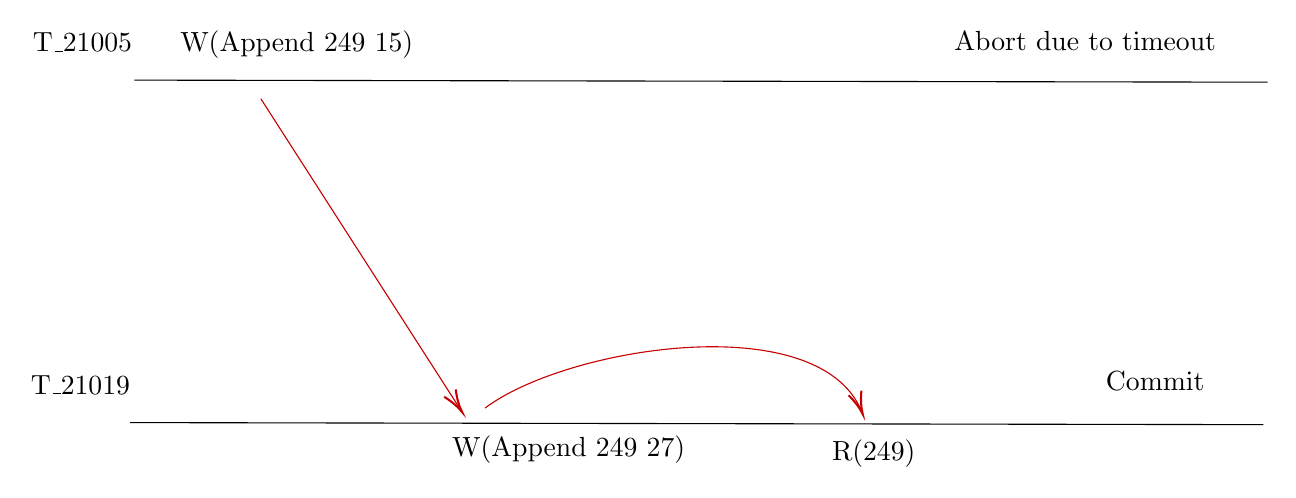
\begin{tikzpicture}[x=0.75pt,y=0.75pt,yscale=-1,xscale=1]
%uncomment if require: \path (0,300); %set diagram left start at 0, and has height of 300

%Straight Lines [id:da9500410641573396] 
\draw    (62.09,31) -- (608.09,32) ;
%Straight Lines [id:da7796185686481738] 
\draw    (60.09,196) -- (606.09,197) ;
%Straight Lines [id:da424831019884359] 
\draw [color={rgb, 255:red, 198; green, 0; blue, 0 }  ,draw opacity=1 ]   (123.09,40) -- (219,189.32) ;
\draw [shift={(220.09,191)}, rotate = 237.28] [color={rgb, 255:red, 198; green, 0; blue, 0 }  ,draw opacity=1 ][line width=0.75]    (10.93,-3.29) .. controls (6.95,-1.4) and (3.31,-0.3) .. (0,0) .. controls (3.31,0.3) and (6.95,1.4) .. (10.93,3.29)   ;
%Curve Lines [id:da475730388715653] 
\draw [color={rgb, 255:red, 198; green, 0; blue, 0 }  ,draw opacity=1 ]   (231.09,189) .. controls (270.69,159.3) and (391.63,140.38) .. (412.48,190.46) ;
\draw [shift={(413.09,192)}, rotate = 249.93] [color={rgb, 255:red, 198; green, 0; blue, 0 }  ,draw opacity=1 ][line width=0.75]    (10.93,-3.29) .. controls (6.95,-1.4) and (3.31,-0.3) .. (0,0) .. controls (3.31,0.3) and (6.95,1.4) .. (10.93,3.29)   ;

% Text Node
\draw (12,7) node [anchor=north west][inner sep=0.75pt]   [align=left] {T\_21005};
% Text Node
\draw (11,172) node [anchor=north west][inner sep=0.75pt]   [align=left] {T\_21019};
% Text Node
\draw (83,6) node [anchor=north west][inner sep=0.75pt]   [align=left] {W(Append 249 15)};
% Text Node
\draw (214,201) node [anchor=north west][inner sep=0.75pt]   [align=left] {W(Append 249 27)};
% Text Node
\draw (397,203) node [anchor=north west][inner sep=0.75pt]   [align=left] {R(249)};
% Text Node
\draw (456,6) node [anchor=north west][inner sep=0.75pt]   [align=left] {Abort due to timeout};
% Text Node
\draw (529,170) node [anchor=north west][inner sep=0.75pt]   [align=left] {Commit};
% Text Node
\draw (120,130) node [anchor=north west][inner sep=0.75pt]   [align=left] {};

\end{tikzpicture}
    
\begin{lstlisting}
{:key 249,
:values [15 27],
:txns [{:type :fail,
        :f :txn,
        :value [[:append 249 15] [:r 251 nil]],
        :time 204766434560,
        :process 18,
        :error Timed out waiting for Shared lock on key;",
        :index 21005}
       ...
       {:type :ok,
        :f :txn,
        :value [[:append 249 27]
                [:r 249 [1 2 3 7 8 11 15 27]]],
        :time 204800363164,
        :process 100,
        :index 21019}]}
\end{lstlisting}

\newpage
\subsubsection{G1a: Aborted Reads (cascaded aborts)}
Aborted reads are common as they share the same underlying issues as Dirty Update, These occur when a transaction commits that it has read the updates of an aborted transaction.\\

The the\todo[author=Jacopo]{the the. Use a grammar checker like grammarly. Errors like this are easy to spot and fix} below example. Transaction 336 wrote to key 2 and afterwards aborted due to being unable to retrieve a lock on key 24. this write was read in Transaction 754 which shouldn't have been possible.


\tikzset{every picture/.style={line width=0.75pt}} %set default line width to 0.75pt        

\begin{tikzpicture}[x=0.75pt,y=0.75pt,yscale=-1,xscale=1]
%uncomment if require: \path (0,300); %set diagram left start at 0, and has height of 300

%Straight Lines [id:da9500410641573396] 
\draw    (62.09,31) -- (608.09,32) ;
%Straight Lines [id:da7796185686481738] 
\draw    (60.09,196) -- (606.09,197) ;
%Straight Lines [id:da424831019884359] 
\draw [color={rgb, 255:red, 198; green, 0; blue, 0 }  ,draw opacity=1 ]   (123.09,40) -- (396.34,191.03) ;
\draw [shift={(398.09,192)}, rotate = 208.93] [color={rgb, 255:red, 198; green, 0; blue, 0 }  ,draw opacity=1 ][line width=0.75]    (10.93,-3.29) .. controls (6.95,-1.4) and (3.31,-0.3) .. (0,0) .. controls (3.31,0.3) and (6.95,1.4) .. (10.93,3.29)   ;

% Text Node
\draw (14,10) node [anchor=north west][inner sep=0.75pt]   [align=left] {T\_336};
% Text Node
\draw (13,175) node [anchor=north west][inner sep=0.75pt]   [align=left] {T\_754};
% Text Node
\draw (85,9) node [anchor=north west][inner sep=0.75pt]   [align=left] {W(append 22 3)};
% Text Node
\draw (216,204) node [anchor=north west][inner sep=0.75pt]   [align=left] {R(23)};
% Text Node
\draw (399,205) node [anchor=north west][inner sep=0.75pt]   [align=left] {R(22)};
% Text Node
\draw (403,10) node [anchor=north west][inner sep=0.75pt]   [align=left] {Abort due to timeout};
% Text Node
\draw (531,173) node [anchor=north west][inner sep=0.75pt]   [align=left] {Commit};
% Text Node
\draw (122,133) node [anchor=north west][inner sep=0.75pt]   [align=left] {};


\end{tikzpicture}


\begin{lstlisting}
    {:op {:type :ok,
        :f :txn,
        :value [[:r 23 [4 5]]
                [:r 22 [1 2 4 3 5 30 32]]],
        :time 10926481665,
        :process 180,
        :index 754},
   :mop [:r 22 [1 2 4 3 5 30 32]],
   :writer {:type :fail,
            :f :txn,
            :value [[:append 22 3]
                    [:append 24 7]],
            :time 6857604069,
            :process 8,
            :error "Timed out waiting for Exclusive lock on key",
            :index 336},
   :element 3}
\end{lstlisting}

\newpage
\subsubsection{G1b: Intermediate Reads (dirty reads)}
Dirty reads occur when a process reads a change prior to this change being committed. 

in the below example.
Transaction 490 writes a change to key 32. this change is then read, and this read is committed prior to 490 committing/aborting.

\tikzset{every picture/.style={line width=0.75pt}} %set default line width to 0.75pt        

\begin{tikzpicture}[x=0.75pt,y=0.75pt,yscale=-1,xscale=1]
%uncomment if require: \path (0,300); %set diagram left start at 0, and has height of 300

%Straight Lines [id:da9500410641573396] 
\draw    (62.09,31) -- (608.09,32) ;
%Straight Lines [id:da7796185686481738] 
\draw    (60.09,196) -- (606.09,197) ;
%Straight Lines [id:da424831019884359] 
\draw [color={rgb, 255:red, 198; green, 0; blue, 0 }  ,draw opacity=1 ]   (123.09,39) -- (175.41,185.12) ;
\draw [shift={(176.09,187)}, rotate = 250.3] [color={rgb, 255:red, 198; green, 0; blue, 0 }  ,draw opacity=1 ][line width=0.75]    (10.93,-3.29) .. controls (6.95,-1.4) and (3.31,-0.3) .. (0,0) .. controls (3.31,0.3) and (6.95,1.4) .. (10.93,3.29)   ;

% Text Node
\draw (13,10) node [anchor=north west][inner sep=0.75pt]   [align=left] {T\_490};
% Text Node
\draw (13,175) node [anchor=north west][inner sep=0.75pt]   [align=left] {T\_553};
% Text Node
\draw (85,9) node [anchor=north west][inner sep=0.75pt]   [align=left] {W(append 32 2)};
% Text Node
\draw (162,203) node [anchor=north west][inner sep=0.75pt]   [align=left] {R(32)};
% Text Node
\draw (298,203) node [anchor=north west][inner sep=0.75pt]   [align=left] {W(append 20 15)};
% Text Node
\draw (354,7) node [anchor=north west][inner sep=0.75pt]   [align=left] {Timeout on key 30};
% Text Node
\draw (531,203) node [anchor=north west][inner sep=0.75pt]   [align=left] {Commit};
% Text Node
\draw (122,133) node [anchor=north west][inner sep=0.75pt]   [align=left] {};
% Text Node
\draw (467,203) node [anchor=north west][inner sep=0.75pt]   [align=left] {R(30)};

\end{tikzpicture}

\begin{lstlisting}
  :G1b ({:op {:type :ok,
        :f :txn,
        :value [[:r 32 [1 2]] 
                [:append 20 15] 
                [:r 30 [5]]],
        :time 18957901065,
        :process 71,
        :index 553},
   :mop [:r 32 [1 2]],
   :writer {:type :fail,
            :f :txn,
            :value [[:append 32 2] 
                    [:append 30 9] 
                    [:r 16 nil] 
                    [:append 30 10] 
                    [:append 32 3]],
            :time 14930759485,
            :process 84,
            :error "System.TimeoutException: Timed out waiting for Exclusive lock on key",
            :index 490},
   :element 2})},
\end{lstlisting}

\newpage
\subsection{Rejected transactions}

One of the symptoms that the reliable collections showed was ever increasing abort rates for transactions containing more than 1 operation, These aborts were caused by heavy deadlocking and timeouts bringing the entire system to a slowdown with test parameters of 200 concurrent clients and randomly distributed transactions with 1-10 sub operations aborting 89.5 \% of the time meaning only 10.5 \% of the transaction got committed.\todo[author=Jacopo]{phrase too long} The reason for these aborts resolves around the way that the API to service fabric is designed, that causing it to be blocking. The reliable collection doesn't preform any query optimizations, or any kind of checks prior to acquiring a lock or attempting to acquire them. 

With 100 concurrent connections the following abort rates were found.. 

\begin{tikzpicture}
\begin{axis}
[
    xlabel={Transaction length}, 
    ylabel={Abort rate in \%}, 
    grid, 
    xmin=0, 
    xmax=11, 
    ymin=0, 
    ymax=100
]
\addplot[red, mark=x, smooth] table[col sep=comma]{results/dataresult.csv};

\end{axis}
\end{tikzpicture}
\subsection{Statistical data from the test.}

Doing the tests some metrics data is gathered. 
\todo[author=Jacopo]{why are you including this data? what are we supposed to look?
Without any description than better to remove them}
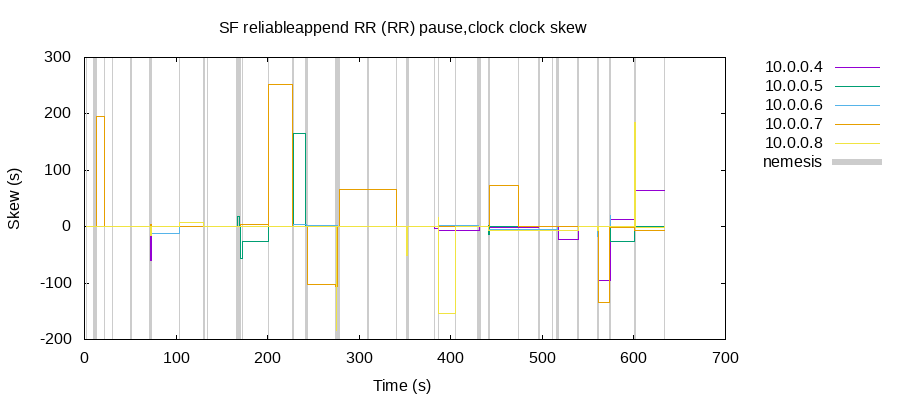
\includegraphics[scale=0.5]{results/clock-skew.png}
\\
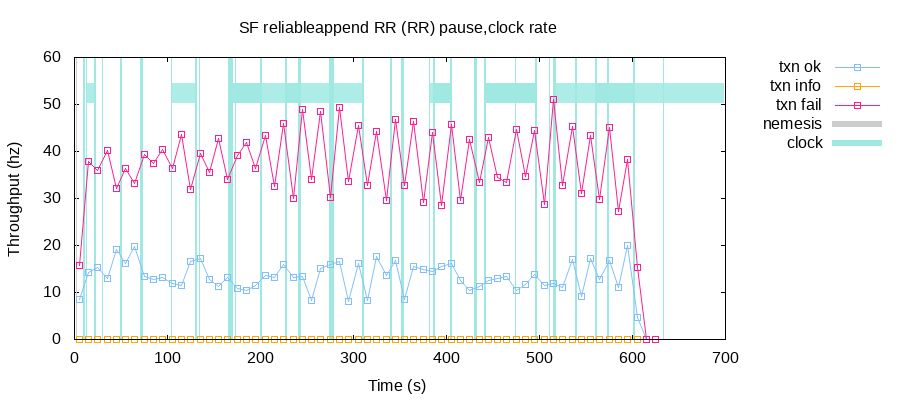
\includegraphics[scale=0.5]{results/rate.png}
\\
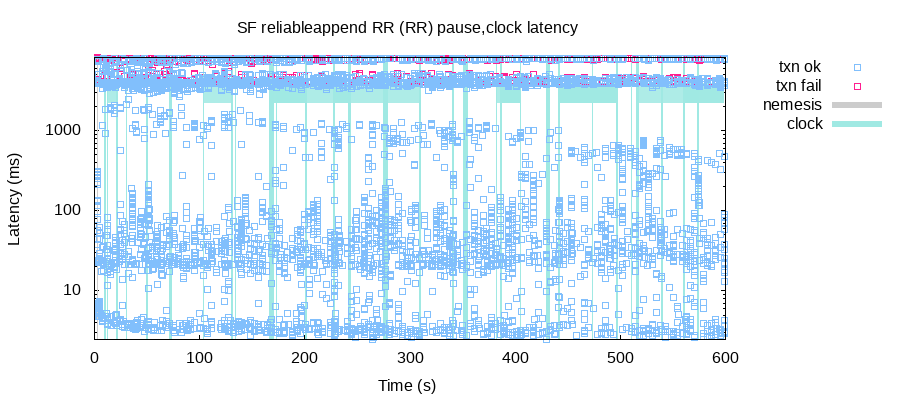
\includegraphics[scale=0.5]{results/latency-raw.png}
\\
\includegraphics[scale=0.5]{results/latency-quantiles.png}


\chapter{Discussion}

Doing this thesis a surprising amount of information was found in existing papers, both concerning databases in general. The lack of precise and unambiguous definitions surrounding them, coupled with the number of database system that violate the consistency models they are presented to follow. This point also applies to service fabric were violations occur with aborted transactions persisting and deadlocks cause a high number of aborts due to the lack of query optimizations within Service Fabric.\\ \vspace{5mm}

    \begin{itemize}
        \item Learning the required tools to implement the services and applications in the first place. C\#, Clojure, and Service Fabric itself as well as reliable collections and lastly Jepsen itself.
        \item Understanding the problem, requirement, topology, architectures and how we want to test these things.
        \item Designing the Services, Libraries, APIs, testing suite, the infrastructure and networking of the cluster and azure.
        \item Implement the Services, Libraries, APIs and testing suite required for things to talk to each other.
        \item Test all the code and configurations and ensure things work as intended.
        \item Execute the test itself.
        \item Analyse the data from the test.
    \end{itemize}
    

\section{Consistency model Standards or the lack thereof}

Doing my time studying prior to this thesis databases were always presented as a fairly strict adhering to strict behavior with predictable results. This turned out to lack a few asterisks where the definitions for databases behavior is ambiguous and often many databases also fail these requirements when they are put under some workloads. Some of the more worrying findings is how often Nosql databases loose data and how often SQL databases violate their set consistency model. This is also not a new discovery either. looking at papers over the past 10 years it is a topic that is being investigated more and more but it also appears that changes are first being made and issues are first resolved often a third party in the open source community brings these issues to light, The paper from Haixiang et al\cite{li2021coo} is one of the more recent papers collecting existing literature on the topics and proposes like many papers prior of defining the Consistency models not in terms of things they prohibit but in unambiguous mathematically notation that cleanly defines what can and can't be expected.\\
\vspace{5mm}
This unambiguous definition would prevent the current situation where databases are presented in the different light compared to how they behave in reality. Currently mislabeling and mis-classification of databases is the norm and when there is no standardized way to classify or test them this issue will persist like aborted reads in Service Fabric, or the other issues discovered while working on the thesis. \\\vspace{5mm}
\begin{itemize}
    \item postgres concerning it's implementation of repeatable read or it's replication functionality.
    \item MongoDB dropping data
    \item Casandra last-write wins issues, %and a attempt at a solution via Atomic clocks
    \item Elastic search issues.
\end{itemize}
\todo[author=Mark]{add some more information to the above points}

All of these issues can have huge implications in the real world if the behavior isn't well understood. Just here in Odense MongoDB is used by the City to gather data from intersections, water usage, water height levels, temperatures, pollution, and many many other things around the city, This implementation might only annoy a few city planners and other city officials but if such a system is used in a place where data is more important such as healthcare or other environment where no data loss is acceptable but due to poor understanding journal data is stored where data critical to human life is lost due to not under the correct understand and information about the system in use.
\todo[author=Mark]{add more to the above concerns.}

\section{How can this be improved going forward}


How to resolve these issues that aeries from mislabeled and misunderstood consistency models.

Enable better understanding of databases, transaction models, and use cases doing teaching of database courses where behavior is better explained, This should not in depth but just to the level of read uncommitted or last-write-wins databases are fine for logging but should be avoided for most systems as they have a lot of unintended behavior, or at least theses systems should be below other layers that ensure that the data is persistent before a commit is accepted.

... should maybe be defined as future work.

Whats next, Defining a standard for testing and certifying database systems towards transactional model that allows the industry to standardize the labelling and allows user and developers to choose the current system for their use case and avoid the headaches of phantom behavior.

This could be done via automated testing and verification of a given system in it's different transactional configurations.


\section{Results from Service Fabric}

\todo[author=Mark]{Email JACOPO when done!}

\chapter{Conclusion and Outlook}
\section*{Conclusion}
\todo[author=Mark]{write Conclusion}

 I will only write deeper about designing, implementing, testing, executing and analysing the results. However this does not mean that the learning and understanding phase of the project was any smaller, quite the contrary. Learning 2 new programming languages that I've never interacted with before isn't an easy task; adding in the complexity of write code for cloud framework that I had no prior experience working on didn't help either. Spicing it with up with outdated documentation, incompatibility between versions of the framework and lack of debugging tools and broken tools meant that a lot was done via eyes blind brute forcing solutions to a lot of issues due to lacking features on the Linux version of the cluster.\\
 
 
Whats next, Defining a standard for testing and certifying database systems towards transactional model that allows the industry to standardize the labelling and allows user and developers to choose the current system for their use-case and avoid the headaches of phantom behavior.

This could be done via automated testing and verification of a given system in it's different transactional configurations.

\section*{Outlook}
\todo[author=Mark]{write Outlook}



\section{Future Work}
\todo[author=Mark]{write Future Work}
Future work could include implementing a deeper testing suite that checks for more types of invariant and issues that might occur in the system.





\newpage


\chapter{Appendix}

\pagestyle{empty}
\printbibliography


\section{Proposal}
\section{'Jepsen methods usage for ACID compliance in Hyperscale Cloud Frameworks'}

\section{Introduction}
The goal of this project is to assess how Jepsen\footnote[1]{https://aphyr.com/tags/jepsen } tests allow us to verify the properties of ACID\footnote[2]{Database Management Systems by Raghu Ramakrishnan \& Johannes Gehrke  ISBN13 9780071231510} in a cloud system.
The Jepsen test is a method used to evaluate the compliance of a system in relation to the ACID properties. This is done is by analysing the system via Blackbox\footnote[3]{https://youtu.be/tRc0O9VgzB0?t=293} tests , in the sense that the internals of the system work are not relevant. We look at the service from a client-side and not any underlying structures or frameworks.
The ACID properties are 
\begin{itemize}
\item	Atomicity \\
Guarantees that each transaction is treated as a single "unit", which either succeeds completely or fails completely 
\item	Consistency \\
Ensures that a transaction can only bring the database from one valid state to another
\item	Isolation \\
Ensures that concurrent execution of transactions leaves the database in the same state that would have been obtained if the transactions were executed sequentially 
\item	Durability \\
Guarantees that once a transaction has been committed, it will remain committed even in the case of a system failure 
\end{itemize}
\footnote[2]{Database Management Systems by Raghu Ramakrishnan \& Johannes Gehrke  ISBN13 9780071231510} \\
We plan to apply these methods on Service Fabric\footnote[4]{https://docs.microsoft.com/en-us/azure/service-fabric/service-fabric-overview  } , to verify if this system is compliant with the ACID properties. Service Fabric is a framework developed by Microsoft, designed to allow developers to build Hyper-Scale Cloud (HSC) deployments on the Azure\footnote[5]{https://microsoft.com/en-us/azure/ } platform.
The motivation behind this thesis is to study the ACID properties in an HSC environment and evaluate how the constraints of ACID hold up in practice, as well as verifying if these constraints are met, and more importantly if they are not. 
\section{Plan}
     
The project is segmented into three parts. The writing of the report will take place at all times throughout the process, and the final phase should be a finalization and corrections phase.  
\subsection{The study phase  }
\begin{itemize}
\item	The first part of the study will focus on analysing the previous\footnote[6]{https://jepsen.io/analyses } Jepsen tests performed on other systems. This will allow us to define a strategy in terms of: which tools, tactics and methods are worth investigating, and what type of faults should be taken note of. This information is useful for two aspects:
\begin{itemize}
\item	where our focus should be when testing,  
\item	which tools and packages we should be familiarize with. 
\end{itemize}
\item	 The second part of the study will centre around “Service Fabric” and getting to know how the framework is coupled together, what vectors we can access the system from, and how we can manipulate the framework to induce fault conditions.   
\end{itemize}
\subsection{The experimentation phase}
\begin{itemize}
\item	In the experimentation phase, we will design and perform tests on the system. If any faults occur, we will attempt to locate where, and why they occur. If the scope and the timeline of the project allow, we will assess whether we prevent the faults from occurring in the future.
\item	The Experimentation phase of the project will include the steps described below. 
\begin{itemize}
\item	Planning of the test, selection of the aspects of the system to be tested, consulting with developers and users of the system to determine if and where undesired behaviour may occur.
\item	Designing the tests and setting up the tools to facilitate those tests.
\item	Writing the tests, verifying they work as intended and setting up a data collection framework to collect the data in a manner that allows our analysis.
\item	Performing the tests on the system in different scenarios, normal conditions and different levels of faults and disaster recovery.
\item	Analysing the data for faults, errors and inconsistencies.
\item	Consulting with DEVs to determine where the faults occurred, and which failures or bugs led to these fault conditions.
\item	Concluding whether “Service Fabric” is ACID-compliant. 
\end{itemize}
\end{itemize}
\subsection{The report phase }
\begin{itemize}
\item The final phase of the project aims at finishing an initial draft, reviewing and correcting it, and finalizing the report for hand-in.
\item	Deliverables 
\begin{itemize}
\item	At the end of the project, there should be a report, the tests and the results from those tests. 
\item	The report written in English and following the standard academic writing conventions will include 
\begin{itemize}
\item	A study on Jepsen tests, describing what they are, as well as why and how they are done.
\item	An experiment in which we will analyse “Service Fabric”	
\item	A discussion on the conclusiveness of the test and the compliance of the framework with service fabric.
\end{itemize}
\item	The code \& data will include
\begin{itemize}
\item	Scripts and code for tests and for analysing the data.
\item	Relevant results and data from the tests. 
\end{itemize}
\end{itemize}
\end{itemize}

\section{Goal}
The goal of the project is to deep dive into Jepsen tests with a focus on “Service Fabric” as the subject. The optimal goal of the project is to verify if the database aspects of “Service Fabric” comply with the ACID properties, and to locate the fault cases in case they don’t.    
Risk assessment 
There are a few risks in the project. In the case no faults are found within the Service Fabric, this reduces the scope of the project. If no faults are found, time allowing, different framework can be analysed. On the contrary, if the number of faults in the framework is more extensive than expected, then the scope of the project may grow uncontrollably. In this case, choices will be made to select a subset of the data to focus on.

\section{TODO}
\todototoc
\listoftodos


    % \section{Schedule}

% Please add the following required packages to your document preamble:
% \usepackage{multirow}
% \usepackage[table,xcdraw]{xcolor}
% If you use beamer only pass "xcolor=table" option, i.e. \documentclass[xcolor=table]{beamer}

    % \begin{tabular}{clll}
    %     \multicolumn{2}{l}{Mark Jervelund thesis plan} & & \\
    %     & Week 45 &                                                    &                                                                                      \\
    %     & Week 46 &                                                    & \multirow{-2}{*}{\text{Study Jensen test}}                                           \\
    %     & Week 47 &                                                    &                                                                                      \\
    %     \multirow{-4}{*}{November} & Week 48 &                                                    & \multirow{-2}{*}{\text{Finish study on Jepsen test}}                                 \\
    %     & Week 49 &                                                    &                                                                                      \\
    %     & Week 50 &                                                    & \multirow{-2}{*}{\text{Study Service Fabric} }                                       \\
    %     & Week 51 &                                                    &                                                                                      \\
    %     & Week 52 &                                                    & \multirow{-2}{*}{\text{Christmas break}}                                             \\
    %     \multirow{-5}{*}{December} & Week 53 &                                                    &                                                                                      \\
    %     & week 01 & \multirow{-10}{*}{\text{Structured study 8 weeks}} & \multirow{-2}{*}{\text{Finish Study Service Fabric} }                                \\
    %     & Week 02 &                                                    &                                                                                      \\
    %     & Week 03 &                                                    & \multirow{-2}{*}{\text{designing the experiment}}                                    \\
    %     \multirow{-4}{*}{January}  & Week 04 &                                                    &                                                                                      \\
    %     & Week 05 &                                                    & \multirow{-2}{*}{\text{designing the experiment} }                                   \\
    %     & Week 06 &                                                    &                                                                                      \\
    %     & Week 07 &                                                    & \multirow{-2}{*}{\text{Execute the experiment}  }                                      \\
    %     \multirow{-4}{*}{February} & Week 08 &                                                    &                                                                                      \\
    %     & Week 09 &                                                    & \multirow{-2}{*}{\text{Analyse the experiment}}                                      \\
    %     & Week 10 &                                                    &                                                                                      \\
    %     & Week 11 & \multirow{-10}{*}{\text{Experiment 10 weeks}}      & \multirow{-2}{*}{\text{discover what the findings from the experiment is}}           \\
    %     & Week 12 &                                                    &                                                                                      \\
    %     \multirow{-5}{*}{March}    & Week 13 &                                                    & \multirow{-2}{*}{\text{Running additional experiments if needed Full on write mode}} \\
    %     & Week 14 &                                                    &                                                                                      \\
    %     & Week 15 &                                                    & \multirow{-2}{*}{\text{Full on write mode} }                                         \\
    %     & Week 16 &                                                    &                                                                                      \\
    %     \multirow{-4}{*}{April}    & Week 17 &                                                    & \multirow{-2}{*}{\text{Full on write mode} }                                         \\
    %     & Week 18 &                                                    &                                                                                      \\
    %     & Week 19 &                                                    & \multirow{-2}{*}{\text{Full on write mode Send out thesis for feedback}}             \\
    %     & Week 20 &                                                    &                                                                                      \\
    %     & Week 21 & \multirow{-10}{*}{\text{Thesis writing 10 weeks}}  & \multirow{-2}{*}{\text{Correction} }                                                 \\
    %     \multirow{-5}{*}{May}      & Week 22 &                                                    &                                                                                      \\
    %     & Week 23 & \multirow{-2}{*}{\text{goal}}                      & \multirow{-2}{*}{\text{Hand in}}                                                     \\
    %     & Week 24 & \multicolumn{1}{l}{}                               & \multicolumn{1}{l}{}                                                                 \\
    %     & Week 25 & \multicolumn{1}{l}{}                               & \multicolumn{1}{l}{}                                                                 \\
    %     & Week 26 & \multicolumn{1}{l}{}                               & \multicolumn{1}{l}{}                                                                 \\
    %     \multirow{-5}{*}{June}     & Week 27 & \multicolumn{1}{l}{}                               & \multicolumn{1}{l}{}                                                                 \\
    %     \multicolumn{1}{l}{}       & Week 28 & \multicolumn{1}{l}{}                               & \multicolumn{1}{l}{}                                                                 \\
    %     \multicolumn{1}{l}{}       & Week 29 & \multicolumn{1}{l}{}                               & \multicolumn{1}{l}{}                                                                 \\
    %     \multicolumn{1}{l}{}       & Week 30 & \multicolumn{1}{l}{}                               & \multicolumn{1}{l}{}                                                                 \\
    %     \multicolumn{1}{l}{}       & Week 31 & \multicolumn{1}{l}{}                               & \multicolumn{1}{l}{}
    % \end{tabular}

\end{document}
